\documentclass[11pt]{article}
  	\usepackage{ucs} 
	\usepackage[utf8x]{inputenc} % Включаем поддержку UTF8  
	\usepackage{babel}  % Включаем пакет для поддержки русского языка 
	\usepackage {mathtext}
	\usepackage{amsmath, amssymb}
	\usepackage{graphicx}
	\usepackage{listings}
	\usepackage{hyperref}
	\usepackage{revsymb}
	\usepackage{listings}
\lstset{language=[90]Fortran,
  basicstyle=\ttfamily,
  keywordstyle=\color{red},
  commentstyle=\color{green},
  morecomment=[l]{!\ }% Comment only with space after !
}
	\hypersetup{
    colorlinks=true,
    linkcolor=blue,
    filecolor=magenta,      
    urlcolor=cyan,
	}
	\urlstyle{same}
	\DeclareGraphicsExtensions{.pdf,.png,.jpg,.jpeg}
	\setcounter{MaxMatrixCols}{20}
	\graphicspath{{pictures/}}
    \title{\textbf{Практическое исследование цепочки Гейзенберга S=1/2 \\ Часть II \\ -- \\ 
	Practical study of the Heisenberg chain S=1/2 \\ Part II}}
    \author{И.А.Юхновский}
    \date{ноябрь 2020}
    
\begin{document}

\maketitle
\thispagestyle{empty}
\section*{Аннотация}
В первой части работы <<Практическое исследование цепочки Гейзенберга S = 1/2>> были рассмотрены теоретические аспекты одномерной спиновой системы, разработан алгоритм расчёта и приведено программное обеспечение на языке Fortran с применением библиотеки многопроцессорных параллельных вычислений openMPI. В данной работе рассматривается практические аспекты построения одномерных спиновых систем.


\section*{Abstract}
In the first part of the work <<Software simulation of the Heisenberg chain S = 1/2>> theoretical aspects of a one-dimensional spin system were considered, a calculation algorithm was developed, and software in the Fortran language was provided using the openMPI multiprocessor parallel computing library. In this second part, we consider practical aspects of constructing one-dimensional spin systems.

\tableofcontents{}

\section{Введение}
Когда тепловые возмущения не зашумляют низкоэнергетические взаимодействия, то появляется возможность наблюдения квантовых кооперативных явлений - волны спиновой и зарядовой плотности, экзотический магнетизм, сверхпроводимость, бозе-эйнштейновская конденсация. Ранее считалось, что данные эффекты возможны только при низких температурах, но с открытием высокотемпературной сверхпроводимости в сложных оксидах переходных металлов, исходно являющиеся антиферромагнитными изоляторами, полностью изменило вектор развития современной физики. Были открыты и стали активно изучаться <<новые магнетики>> - вещества с пониженной размерностью магнитной подсистемы и фрустрацией обменного взаимодействия, где основным состоянием является спиновая жидкость, а свойства близки к электронной жидкости в сверхпроводниках. Была открыта важная роль в формировании сверхроводимости магнитной подсистемы. Новый или низкоразмерный магнетизм проявляется во фрустрированных системах, когда формирование дальнего магнитного порядка затруднено или оказывается невозможным. Первыми были открыты оксиды меди, затем пниктиды и халькогениды железа - достаточно большой список приведен в ~\cite{mp}. Данные открытия сформировали новые направления в физике конденсированного состояния: физика спиновых жидкостей, неколлинеарных и экзотических магнитных структур, топологических изоляторов, мультиферроэлектричества и квантовой суперпозиции состояний.

В области низкоразмерного магнетизма активно ведется поиск и улучшение функциональных параметров новых магнитных соединений, приведением их характеристик в соответствие с технологическими требованиями производства. 

В данной работе рассматриваются одномерные системы, поскольку существуют теоретические модели, на основании которого стало возможным разработка программного обеспечения. В квазиодномерных системах как <<наиболее яркий эффект , ответственный за формирование квантовых основных состояний>> в ~\cite{nm} выделяют спин-пайерловский переход и формирование спин-синглетного состояния за счет зарядового и орбитального упорядочений. Также, отмечается, что <<палитра физических явлений в двумерных магнитных системах гораздо богаче, нежели в одномерных>> ~\cite{nm}стр.281, однако теоретические модели ~\cite{nm} и программный рассчет усложняются значительно. Был сделан выбор в пользу одномерных систем, поскольку качественная проверка гипотезы управляемого влияния ионизационного излучения на низкомерный магнетик проще сделать на более простой теоретической и вычислительной модели. В развитии одномерной модели, были рассмотрены и спиновые лестницы. Данные по структурам кристаллических решеток были взяты из открытых источников:
\begin{itemize} 
\item American Mineralogist Crystal Structure Database (AMCSD)  ~\footnote{~\url{http://rruff.geo.arizona.edu/AMS/amcsd.php}} 
\item Cambridge Structural Database (CSD) ~\footnote{~\url{http://www.ccdc.cam.ac.uk/products/csd/}}
\item Crystallography Open Database (COD) ~\footnote{~\url{https://en.wikipedia.org/wiki/Crystallography_Open_Database}}
\item Crystallography Online (Web Interface for COD) ~\footnote{~\url{http://crystallography-online.com/}}
\item Database of Zeolite Structures ~\footnote{~\url{http://www.iza-structure.org/databases/}}
\item Incommensurate Structures Database ~\footnote{~\url{http://www.cryst.ehu.es/icsdb/index.html}}
\item Inorganic Crystal Structure Database (ICSD) ~\footnote{~\url{https://en.wikipedia.org/wiki/Inorganic_Crystal_Structure_Database}}
\item MaterialsProject Database ~\footnote{~\url{http://materialsproject.org/}}
\item MaterialsWeb Database ~\footnote{~\url{http://materialsweb.org/}}
\item Metals Structure Database (CRYSTMET) ~\footnote{~\url{https://web.archive.org/web/20080622165920/http://tothcanada.com/databases.htm}}
\item Mineralogy Database ~\footnote{~\url{http://webmineral.com/}}
\item MinCryst ~\footnote{~\url{http://database.iem.ac.ru/mincryst/index.php}}
\item NIST Structural Database NIST Structural Database  ~\footnote{~\url{https://web.archive.org/web/20080516022153/http://www.nist.gov/srd/nist83.htm}}
\item NIST Surface Structure Database ~\footnote{~\url{https://web.archive.org/web/20080610153131/http://www.nist.gov/srd/nist42.htm}}
\item Pearson's Crystal Data ~\footnote{~\url{http://www.crystalimpact.com/pcd/Default.htm}}
\item Wiki Crystallography Database (WCD)  ~\footnote{~\url{http://nanocrystallography.research.pdx.edu/search/wcd/}}
\end{itemize} 

Цель работы - подготовить экспериментальную базу для исследования влияния ионизационного излучения на новые магнетики для изучения возможности построения квантового компьютера в инфраструктуре ядерного топливного цикла. 

Эксперимент на первом этапе будет заключаться в использовании магнитных систем в качестве мишеней облучения для различных источников ионизационного излучения, измерения изменений электрических и магнитных характеристик мишени, измерении сечений в зависимости от теплофизических и электро-магнитных состояний материала мишени. 

 На втором этапе можно будет попробовать построить химические соединения на радиоактивных изотопах, смеси магнетика и радиоактивного источника, конфигурации слоев магнетика и радиоактивного материала источника (по аналогии со слоями в процессоре) с целью усиления фрустрационных эффектов. Исследовать полученные материалы на изменение свойств спиновой системы при нормальных и высоких температурах. Последнее видятся перспективными с точки зрения размещения квантового компьютера внутри или в непосредственной близости от активной зоны реактора.

\section{Квазиодномерные магнетики}
\subsection{Однородная цепочка получисленных спинов}
В подавляющем большинстве квазиодномерных соединений с болшьшими величинами констант обменного взаимодействия при некоторой температуре происходит трехмерное упорядочение из-за межцепочечного взаимодействия 
\subsubsection{Молибдат рубидия-меди}
Низкоразмерная структура и магнетизм квантовго антиферромагнетика $Rb_4Cu(MoO_4)_3$ была изучена и опубликована в ~\cite{ishii2010}.

\begin{figure}[htp]
\centering
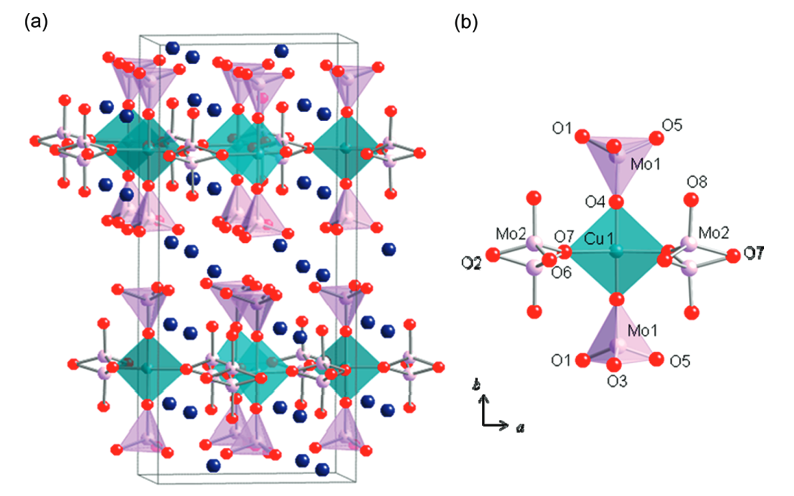
\includegraphics[scale=0.55]{Rb_4Cu_MoO_4}
\caption{Структура кристалла $Rb_4Cu(MoO_4)_3$ $Rb$-голубой, $Cu$-зеленый, $Mo$-фиолетовый, $O$-красный ~\cite{ishii2010}}
\label{}
\end{figure}

$Rb_4Cu(MoO_4)_3$ наиболее ярко иллюстрирует свойства однородной антиферромагнитной гейзенберговской цепочки. 

Соединение при комнатной температуре обладает орторомбической кристаллической решеткой, пространственной группы $Pnma$ ~\cite{ishii2010}. В нем магнитоактивные ионы меди $Cu^{2+}$ $(d_{x^2-y^2}, S=1/2)$ находятся в пирамидальном окружении кислородных анионов. Пирамиды соединенные между собой $MoO_4$ группами, формируют двумерные плоскости $ac$, при этом магнитные пирамиды могут взаимодействовать между собой через промежуточные молибденовые группы. 

\subsubsection{Диацетат ванадила}
Диацетат ванадила $VO(CH_3COO)_2$ имеет нецентросимметричную $Cmc2_1$ пространственную группу ~cite{weeks2003}.

\begin{figure}[htp]
\centering
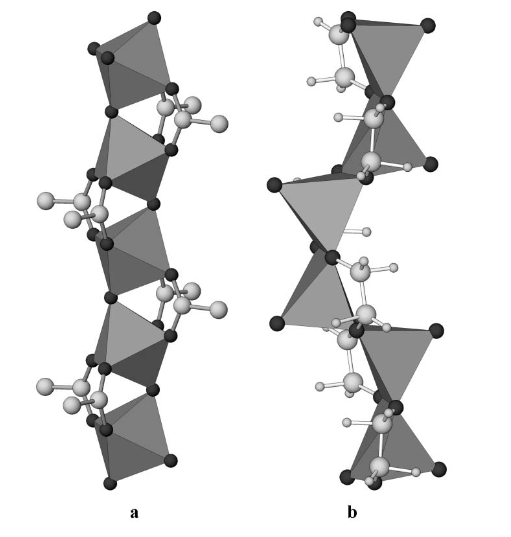
\includegraphics[scale=0.55]{VOCH3COO}
\caption{a) Одномерная цепочка октаэдров $V)_6$ в структуре $VO(CH_3COO)_2$ b) одномерная цепочка квадратных пирамид $VO_5$ в структуре $VO(CH_3COO)_2$ ~\cite{weeks2003}}
\label{}
\end{figure}

В структуре содержаться квадратные пирамиды $VO_5$, связанные между собойчерез апикальные кислороды, тем самым образуя слои из бесконечных одномерных цепочек. Магнитоактивные цепочки в структуре диацетата ванадила находятся далеко друг от друга, что предполагает слабую магнитную связь между ними.

Первопринципные теоретические рассчеты основных обмменных взаимодействий были выполнены в ~\cite{koo2010}

Исследования показали, что в магнитной цепочке присутствуют как суперобменные спиновые взаимодействия $V-O-V$, так и суперсуперобменные взаимодействия через ацетатные группы по пути $V-O \cdot \cdot \cdot O-V$ и при этом они оказываются доминирующими.
Основной обмен - антиферромагнитный, осуществляется через углеродную $2p_{\pi}$ орбиталь ацетатного иона $[CH_3COO]^{-}$

\subsection{Однородная цепочка с конкурирующими взаимодействиями}
Является усложнением модели однородной цепочки Гейзенберга, где к обменным взаимодействиям между соседями $J_1$ добавляются взаимодействия со следующим за ближайшим соседом $J_2$. Это может приводить к фрустрации и появлению новых основных состояний.

\subsubsection{Цирконат лития-меди}
На рисунке ниже приведен фрагмент элементарной ячейки $\gamma - Li_2CuZrO_4$ , в которой ионы меди формируют ленты из соединенных по ребру квадратов $CuO_4$, угол связи составляет 94°, что 
отвечает ферромагнитному обмену и довольно близко к критическому значению угла связи 96°, разделяющему ферро- и антиферромагнитное обменные взаимодействия ~\cite{goodenough}.
Ионы $Li$ занимают две позиции, причем одна из них нажодится между слоями $Cu-Li$, наполовину заполнена и подвижна.
Для установления температуры магнитного упорядочения в системе $\gamma - Li_2CuZrO_4$ были выполнены детальные низкотемпературные измерения магнитной восприимчивости, теплоемкости и спектров рассеяния мюонов, которые показали, что максимум зависимости магнитной восприимчивости от температуры $\xi(T)$ при 8К не соответствует формированию магнитоупорядоченного состояния, тогла как дальний магнитный порядок возникает при более низкой температуре $T_N=6,8K$, при которой демонстрируют анамалию температурные зависимости производной магнитной восприимчивости $d\xi/dT$, теплоемкость $C_p$ и поперечная скорость релаксации мюонов.
В ~\cite{jpscp_8_034012} приводятся результаты расчета энергетического спектра методом локальной спиновой аппроксимации (LSDA+FPLO) и оценка обменных магнитных взаимодействия. Данные нейтронной дифракции, выполненной на порошколвом образце $Li_2CuZrO_4$ дают оценку $\Delta \phi = 88°$ и $\alpha=6,2$, что ставит это соединение далеко от квантовой критической точки.


\begin{figure}[htp]
\centering
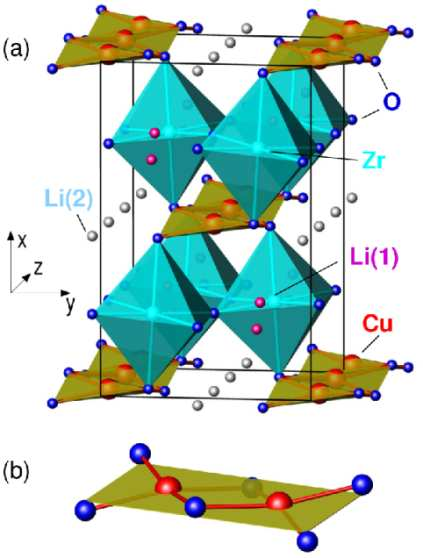
\includegraphics[scale=0.55]{Li2ZrCuO4}
\caption {Элементарная ячейка $\gamma - Li_2CuZrO_4$ ~\cite{schmitt2009}}
\label{}
\end{figure}



\subsubsection{Изоструктурные купраты лития и натрия}
Кристаллы $LiCu_2O_2$ и $NaCu_2O_2$ имеют орторомбическую симметрию, пространственная группа Pnma ~\cite{tams}. Параметры кристаллической решетки оказались связаны соотношением $a \approx 2b$, что приводит к двойникованию при росте кристаллов и сложностям в их ориентировании ~\cite{maljuk2004}. \\

Так как ионные радиусы $Li^+$, $Cu^{+}, Cu^{2+}$ близки, то может происходить замещение $Li$ позиций $Cu$, в отличии от купрата натрия, поскольку ионный радиус $Na^{+}$ значительно больше. \\

При исследовании свойств $LiCu_2O_2$ и $NaCu_2O_2$ качество монокристаллов и присущий химический беспорядок играют ключевую роль и приводят к существенному разбросу экспериментальных данных ~\cite{nm}. \\

У этих купратов в структуре есть два катиона $Cu$ со степенями окисления +1 и +2 в пропорции $1:1$. Такая структура моделируется как последовательное чередование трех слоев:
\begin{itemize} 
\item $-Li/Na - O - Cu^{2+} - O -$
\item $- Cu^{+} -$
\item $- O - Cu^{2+} - O - Li/Na -$
\end{itemize} 

\begin{figure}[htp]
\centering
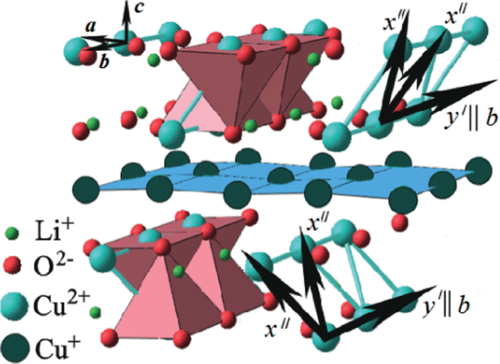
\includegraphics[scale=0.7]{LiCu2O2}
\caption {Орторомбическая кристаллическая структура $LiCu_2O_2$ ~\cite{seidov2017}}
\label{}
\end{figure}

\begin{figure}[htp]
\centering
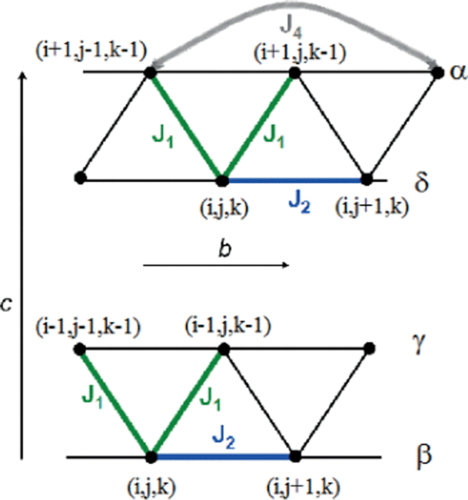
\includegraphics[scale=0.7]{LiCu2O2_1}
\caption {Схематическое отображение обменного взаимодействия между магнитными ионами меди $Cu^{2+}$ в $LiCu_2O_2$. Индексы $i,j,k$ соответствуют кристаллографическим осям на ~\cite{seidov2017}}
\label{}
\end{figure}


\begin{figure}[htp]
\centering
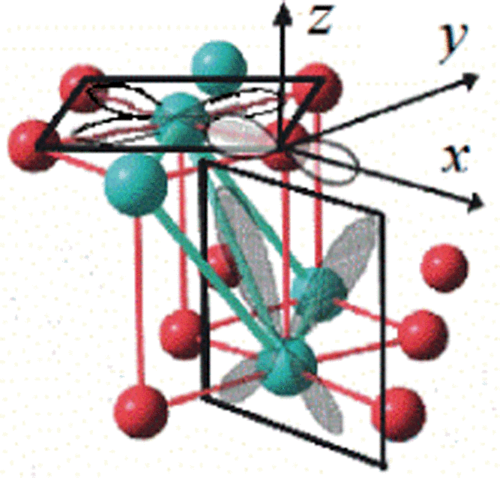
\includegraphics[scale=0.7]{LiCu2O2_2}
\caption {Схематический путь возникновения анизотропной спиновой связи $A_{yy}$ между медью (голубые большие сферы) в состоянии $d_{x^2-y^2}$ и с медью в возбужденном состоянии(серыый) через кислород(красный)  в $LiCu_2O_2$. Индексы $i,j,k$ соответствуют кристаллографическим осям на ~\cite{seidov2017}}
\label{}
\end{figure}

\begin{figure}[htp]
\centering
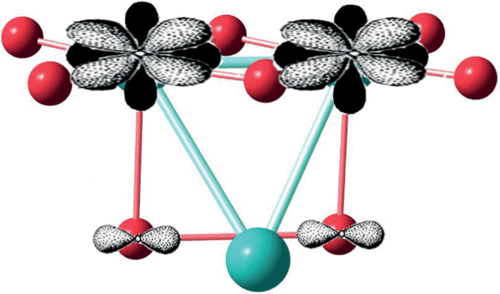
\includegraphics[scale=0.7]{LiCu2O2_3}
\caption {Возможный путь реализации антисимметричной анизотропной $(DM)$ обменной связи $D_2$ между соседними ионами меди внутри цепочек в $LiCu_2O_2$ ~\cite{seidov2017}}
\label{}
\end{figure}

\begin{figure}[htp]
\centering
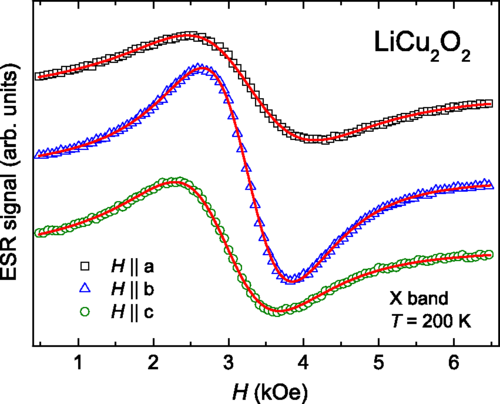
\includegraphics[scale=0.7]{LiCu2O2_4}
\caption {Типичные спектры ESR $LiCu_2O_2$ для магнитных полей приложенных вдоль трех основных кристаллографических осей ~\cite{seidov2017}}
\label{}
\end{figure}

На основе нейтронографических исследований, проведенных в работе   , для купрата литиябыло установлено, что каждая из двух спиновых цепочек выстраивается в спиральную структуру, в которой спины лежат в параллельных плоскостях $ab$ и совмещаются друг с другом посредством вектора $\vec q = (1/2,k,0)$, где $k$ играет рольпараметра несоизмеримости периода решетки с периодом магнитной спирали. 

\begin{figure}[htp]
\centering
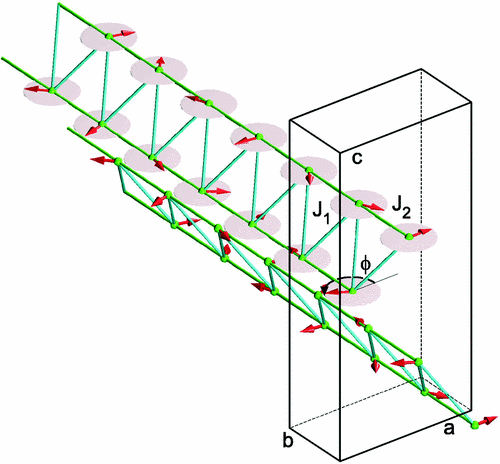
\includegraphics[scale=0.7]{LiCu2O2_5}
\caption {Элементарная ячейка $LiCu_2O_2$ ~\cite{masuda2004} (ионы меди показаны сферами) и планарная геликоидальная магнитная структура при T=2K (направления магнитных моментов показаны стрелками)}
\label{}
\end{figure}

Полученные результаты исследований относят $LiCu_2O_2$ к мультиферроикам, который может служить прототипом ферроэлектрика с одномерной спиральной магнитной структурой.


\subsubsection{Фосфат рубидия-меди-алюминия}
Кристаллическая структура фосфата рубидия-меди-алюминия $RbCuAl(PO_4)_2$ является моноклинной и имеет пространственную группу $P2_1/c$ ~\cite{yakubovich2016}.

\begin{figure}[htp]
\centering
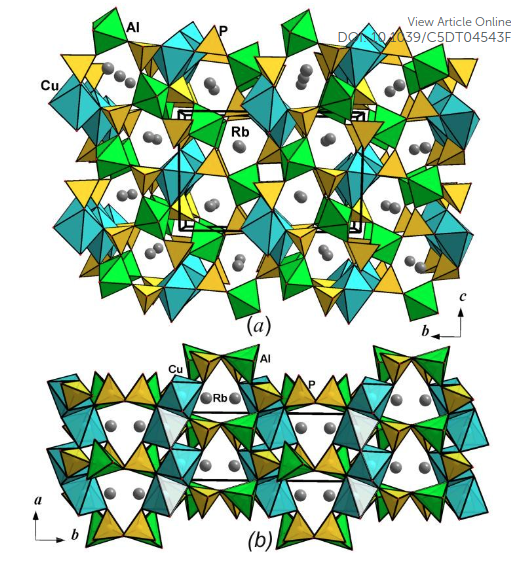
\includegraphics[scale=0.7]{RbCuAlPO42}
\caption {Структура $RbCuAl(PO_4)_2$ ~\cite{yakubovich2016} (a) - ось а, (b) - ось с}
\label{}
\end{figure}

Нецентросимметричная структура содержит слои зигзагообразных цепочек сильноискаженных октаэдров $CuO_6$, связанных по ребру. Цепочки пространственно разделены друг от друга тетраэдрами фосфора $PO_4$ и бипирамидами алюминия $AlO_5$. При этом в элементарной ячейке формируются открытые каналы параллельно осям $a$ и $c$, в которых располагаются ионы $Rb^{+}$. Октаэдры $CuO_6$ сильно искажены в соответствии с эффектом Яна-Теллера ~\footnote{совокупность эффектов, связанных с взаимодействием орбитальных состояний электронов и искажений поля кристаллической решётки} ~\cite{bersuker}, характерным для ионов меди $Cu^{2+}(d^9)$. Магнитная подсистема представлена цепочками связанными по ребру октаэдров в сочетании со слабыми межцепочечными взаимодействиями через полиэдры $PO_4$ и $AlO_5$. Поскольку внутри цепочек октаэдры $CuO_6$ чередуются через $cis-$ и $trans-$ связи, то возникают обмены как антиферро-, так и ферро-магнитного типа, подобно ситуации, которая наблюдается в пироксенах ~\cite{isobe2002}.
В {nm} приведены параметры обменных взаимодействий.

\subsubsection{Ванадил-дифосфат цезия-меди}
$CsCu(VO)(P_2O_7)_2$ характеризуется нецентросимметричной орторомбической кристаллической структурой с пространственной группой $Pn2_1a$ ~\cite{shvanskaya2015}

\begin{figure}[htp]
\centering
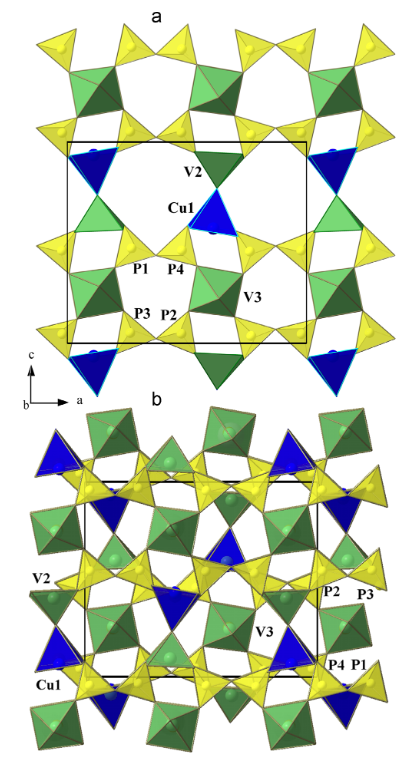
\includegraphics[scale=0.7]{CsCuVOP2O72_1}
\caption {Структура $CsCu(VO)(P_2O_7)_2$ в проекции (0 1 0) ~\cite{shvanskaya2015}}
\label{}
\end{figure}

\begin{figure}[htp]
\centering
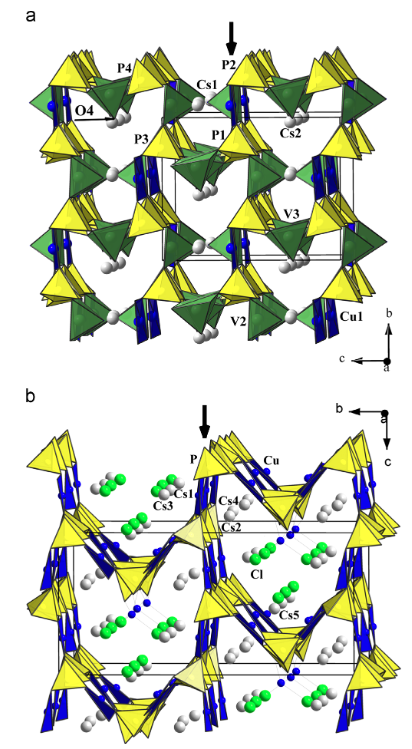
\includegraphics[scale=0.7]{CsCuVOP2O72_2}
\caption {Структура $CsCu(VO)(P_2O_7)_2$ в проекции (1 0 0) ~\cite{shvanskaya2015}}
\label{}
\end{figure}

Структура формируется ионами $Cu$ в квадратно-пирамидальном окружении, тетрагональными пирамидами $VO_5$ и дифосфатными группами $P_2O_7$, связанными как $Cu-O-V$, $Cu-O-P$ и $V-O-P$. Эти группы формируют открытые каналы для ионов цезия. В элементарной ячейке присутствуют по три кристаллографически независимых позиции для магнитных ионов меди и ванадия.

\begin{figure}[htp]
\centering
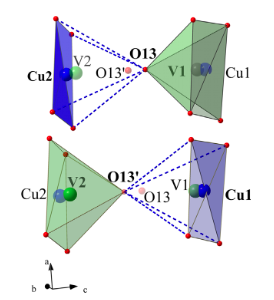
\includegraphics[scale=0.7]{CsCuVOP2O72_3}
\caption {Две возможные конфигурации в расположении ионов $Cu, V, O$  ~\cite{shvanskaya2015}}
\label{}
\end{figure}

$Cu1$ и $Cu2$ немного выходят из базальной плоскости квадратных кислородных пирамид, а ионы $Cu3$ находятся в плоско-квадратном окружении. 

Магнитные ионы $V^{4+}$ координированы пятью ионами кислорода в квадратную пирамиду с одним кратчайшим расстоянием $V-O$, что характерно для ванадильных групп. При этом ионы $V^{4+}$ смещены из базальной плоскости в направлении вершины пирамиды и формируют димеры с ионами $Cu^{2+}$. Связанные по углу квадратные пирамиды ванадия, меди и дифосфатные группы формируют сотообразные слои параллельные плоскости $ac$ ~\cite{nm}.

Поскольку в исследуемой системе присутствуют два магнитных иона:
\begin{itemize} 
\item  $Cu^{2+}(d^9, S=1/2)$
\item  $V^{4+}(d^1, S=1/2)$
\end{itemize} 

то им соответствуют две резонансные моды со средними эффективными значениями $g-$факторов при комнатной температуре: 

\begin{itemize} 
\item $g_1=2,001$
\item $g_2=2,037$
\end{itemize} 

Принимая во внимание присутствие трех неэквивалентных позиций для пар меди и ванадия, Cu1/V1, Cu2/V2 и Cu3/V3, спектр ЭПР такой концентрированной магнитной системы представляет собой суперпозицию статически усредненных мод, отвечающих отклику парамагнитных центров $Cu^{2+}$ и $V^{4+}$, которые связаны обменным взаимодействием.

В первом приближении теории возмущений спиновый гамильтониан для двух различных $S=1/2$ спинов $i$ и $j$ с различными $g-$факторами и изотропным обменным взаимодействием $J$ может быть записан как:

$\hat H = \mu_BB_z(g_{iz}S_{iz} + g_{iz}S_{jz})+ J(S_i \cdot S_j) $

, где $B_z$ - магнитное поле вдоль оси $z$ (основная ось анизотропии для двух $g-$тензоров),  $\mu_B $ - магнетон Бора. В остутствии обменного взаимодействия между спинами $i$ и $j$ (аналогично случаю изолированных ионов) переход возникает при: 

\begin{itemize} 
\item $h\nu = g_{iz}\mu_BB_z $ 
\item $h\nu = g_{jz}\mu_BB_z $ \\
\end{itemize} 

Когда взаимодействие достаточно слабое наблюдаются для разрешенных переходов два дублета :
\begin{itemize} 
\item $(|++\rangle \leftrightarrow |-+\rangle)$ и $(|--\rangle \leftrightarrow |+-\rangle)$
\item $(|++\rangle \leftrightarrow |+-\rangle)$ и $(|--\rangle \leftrightarrow |-+\rangle)$
\end{itemize} 

Расстояния между резонансными модами в каждом дублете в первом приближении равно обменной энергии $J$

С ростом обменного взаимодействия переходы
\begin{itemize} 
\item $(|--\rangle \leftrightarrow |+-\rangle)$
\item $(|--\rangle \leftrightarrow |-+\rangle)$
\end{itemize} 

расходятся и ослабевают по амплитуде, тогда как

\begin{itemize} 
\item $(|++\rangle \leftrightarrow |-+\rangle)$
\item $(|++\rangle \leftrightarrow |+-\rangle)$
\end{itemize} 

смещаются к центральной частоте: \\

$h\nu = \frac{1}{2}(g_{iz}+g_{jz})\mu_BB_z$ \\

а их интенсивность значительно растет, так что при определенном значении обменного параметра в спектре наблюдается лишь две внутренние моды. В этом случае, значения эффективных $g-$факторов могут существенно отклоняться от значений, ожидаемых на основании теории кристаллического поля данной координации лигандов ~\cite{nm} стр.79.

\subsubsection{Селенит-оксохлорид висмута-железа}
Кристаллическая структура $Bi_2Fe(SeO_3)_2OCl_3$ слоистая моноклинная с пространственной группой $P2_1/m$ ~\cite{berdonosov2014}. Основная особенность кристаллической структуры - присутствие изолированных зигзагообразных цепочек ионов $Fe^{3+} (S=5/2)$ вдоль оси $b$, сформированных связанными по углу октаэдрами $FeO_6$, окруженными немагнитными группами $BiO_4Cl_3$, $BiO_3Cl_3$ и $SeO_3$.

\begin{figure}[htp]
\centering
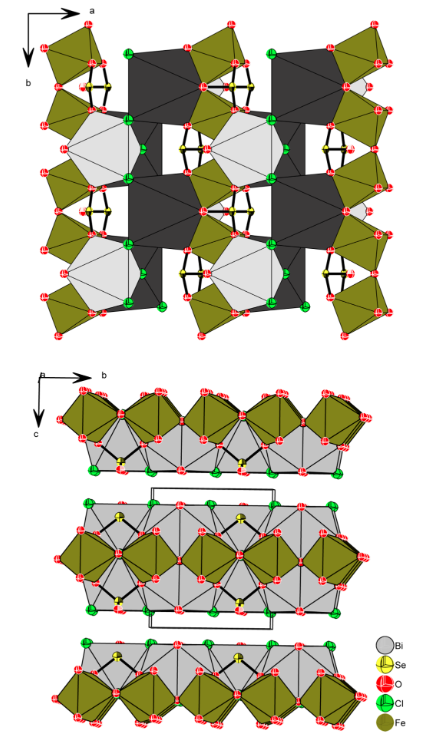
\includegraphics[scale=0.7]{Bi2FeSeO32OCl3}
\caption {Структура $Bi_2Fe(SeO_3)_2OCl_3$  ~\cite{berdonosov2014}}
\label{}
\end{figure}

В спектрах ЭПР наблюдается одиночная обменно-суженная линия, повидимому, отвечающая сигналу ионов $Fe^{3+}$ в малоискаженной октаэдрической кислородной координации. Наблюдаются две резонансные моды, которые различаются по интенсивности: основной вклад в поглощение вносит намного более интенсивная мода $L_1$, тогда как вклад компоненты $L_2$ менее 2\% и связан с наличием небольшого количества примеси в образце. Доминирующее взаимодействие - суперобмен в цепочке связанных по углу октаэдров $FeO_6$. Взаимодействие через апикальные кислороды - антиферромагнитные как для 90°, так и для 180° углая связи $Fe^{3+} - O^{2-} - Fe^{3+}$ Таким образом, антиферромагнитные цепочки спинов $S=5/2$ с обменным интегралом $J_{||}$ определяют магнитное поведение $Bi_2Fe(SeO_3)_2OCl_3$ с широким корреляционным максимумом на $\xi(T)$ при высоких температурах.~\cite{nm}

\subsection{Альтернированная цепочка}
Альтернированную (чередующуюся) цепочку можно изобразить в виде схемы: \\

o---$J_1$---o......o---$\alpha J_1$--o ...... o------o \\
 
и описывается тремя эквивалентными гамильтонианами ~\cite{johnston2000}

$\hat H = \sum_iJ_1 \vec S_{2i-1} \vec S_{2i} + J_2 \vec S_{2i} \vec S_{2i+1} = $ 
 
$\sum_i J_1 \vec S_{2i-1} \vec S_{2i} + \alpha J_1 \vec S_{2i} \vec S_{2i+1} = $ 
 
$\sum_i J(1+\delta ) \vec S_{2i-1} \vec S_{2i} + J(1-\delta ) \vec S_{2i} \vec S_{2i+1}$  
 
где: \\
 
$J_1=J(1+\delta) = \frac{2J}{1+\alpha}$ \\

$J = \frac{J_1+J_2}{2} = J_1\frac{1+\alpha}{2}$ \\
 
$\alpha=\frac{J_2}{J_1}=\frac{1-\delta}{1+\delta} $\\
 
$\delta=\frac{J_1}{J}-1 = \frac{J_1-J_2}{2J} = \frac{1-\alpha}{1+\alpha}$ \\
 
с антиферромагнитными взаимодействиями $J_1 \ge J_2 \ge 0$ и параметрами альтернирования $ 0 \le \alpha, \delta \le 1 $. 
 
Для значений параметра альтернирования $0 \le \alpha \le 0,9$ величина спиновой щели $\Delta$ ~\cite{johnston2000}: \\

$\Delta^{*}(\alpha) = \frac{\Delta(\alpha)}{J_1} = (1-\alpha)^{3/4}(1+\alpha)^{1/4}$ \\

$\Delta^{*}(\delta) = \frac{\Delta (\delta)}{J} = 2\delta^{3/4}$ \\

Тамже были получены  в одномагнонном приближении  зависимости теплоемкости и магниной восприимчивости при $T \rightarrow 0 $.

Соединение $(VO)_2P_2O_7$ содержит две близко расположенных цепочки магнитных ионов $V^{4+}$ - два вида алтернированных спиновых цепочек. $(VO)_2P_2O_7$ обладает моноклинной кристалличческой структурой с пространственной группой $P2_1$. Элементарная ячейка содержит восемь неэквивалентных позиций для ванадия и фосфора. Алтернированные цепочки направлены вдоль оси $b$, каждая из них содержит пары связанных по ребру $VO_5$ пирамид, которые разделены $PO_4$ тетраэдрами ~\cite{nguyen1995}.

\begin{figure}[htp]
\centering
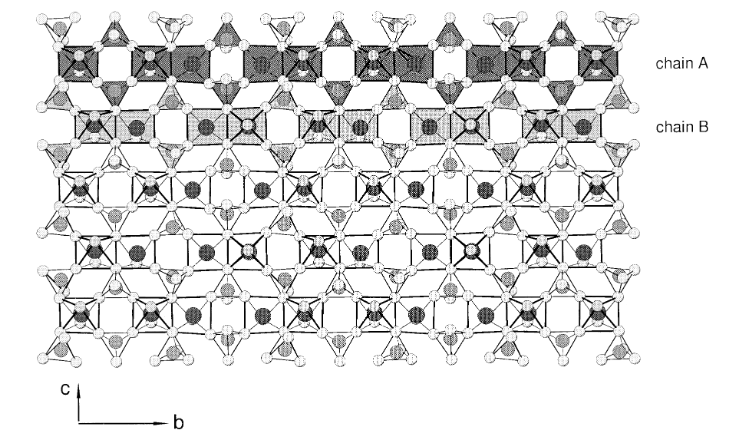
\includegraphics[scale=0.5]{VO2P2O7}
\caption {Структура $(VO)_2P_2O_7$  ~\cite{haras2002}}
\label{}
\end{figure}


При самых низких температурах в спектрах $^{31}P$ ядерного магнитного резонанса $(VO)_2P_2O_7$ был найден пик, отвечающий немагнитному основному состоянию. С увеличением температуры этот пик смещался и расщеплялся сначала на две, а затем на четыре лини. То есть восемь позиций фосфора разделяются на четыре группы, которые чувствуют различные внутренние поля, создаваемые ионами ванадия. Затем при самых высоких температурах в спектре вновь наблюдается лишь идин пик. Смещение и немонотонное изменение амплитуд отдельных линий при повышении температуры указывает на наличие нескольких спиновых компонент с различными температурными зависимостями магнитной восприимчивости. ~\cite{nm}

В экспериментах по неупругому рассеянию нейтронов ~\cite{garrett1997} были обнаружены две дисперсионные кривые и соответственно две щели. Обе кривые указывают на большую величину параметра антиферромагнитного обмена вдоль оси $b$. Об этом также свидетельствует полевая зависимость намагниченности.

\begin{figure}[htp]
\centering
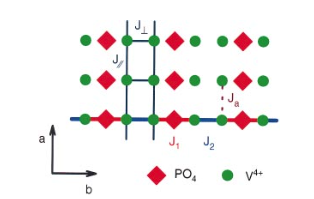
\includegraphics[scale=0.8]{VO2P2O7_1}
\caption {Взаимодействия в $VOPO$  ~\cite{garrett1997}}
\label{}
\end{figure}


\subsection{Спин-пайерловский переход}
Спин-пайерловский переход возникает при понижении температуры, когда квазиодномерная структура испытывает фазовый переход с удвоением периода кристаллической решетки, что отвечает проигрышу в энергии упругой подсистемы, но открывается щель в спектре магнитных возбуждений, что эквивалентно выигрышу в энергии магнитной подсистемы. Детально исследованным металлоксидом, испытывающим спин-пайлеровский переход является $CuGeO_3$. Этот переход возникает в кристаллах, содержащих изолированные однородные цепочки полуцелочисленных спинов. Такие цепочки не имеют щели в спектре магнитных возбуждений, однакок, общая энергия кристалла может быть понижена за счет алтернирования обменного взаимодействия.
Соединение $CuGeO_3$ имеет орторомбическую структуру с пространственной группой $Pbmm$. Цепочки октаэдров $CuO_6$ и разделяющие их цепочки тетраэдров $GeO_4$ расположены вдоль оси $с$. Носителями магнитного момента $S=1/2$ cke;fn bjys $Cu^{2+}$  с незаполненной d-оболочкой. ~\cite{nm}

Спин-пайерлсовский переход был обнаружен в $CuGeO_3$ в измерениях магнитной восприимчивости на монокристаллах ~\cite{hase1993}.

\begin{figure}[htp]
\centering
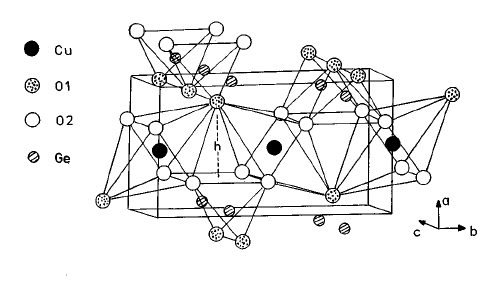
\includegraphics[scale=0.5]{CuGeO3}
\caption {Структура $CuGeO_3$  ~\cite{krishnamurthy1997}}
\label{}
\end{figure}

С понижением температуры при $T_M \sim $ 56K наблюдался корреляционный максимум, а при $T_{SP} \sim $14K вдоль всех кристаллографических направлений наблюдалось резкое уменьшение магнитной восприимчивости. Обработка зависимости при $\chi(T)$ при высоких температурах в модели однородной цепочки полуцелочисленных спинов $S=1/2$ позволяет оценить интеграл обменного взаимодействия вдоль цепочки как $J_C \sim $ 88K.

Самоорганизация несоизмеримой фазы спин пайерловских магнетиков наблюдалось в рентгенографических исследованиях по появлению дополнительного периода кристаллической решетки в виде солитонов с полушириной $\sim$ 13,6 периода решетки.

Исследования магнитострикции и коэффициентов теплового расширения в магнитных полях показали, что решетка солитонов при приближении к границе фаз I-U перестраивается в синусоидальную модуляцию ~\cite{lorenz1998}.

\subsection{Орбитальный механизм димеризации спиновой цепочки}
Однородные антиферромагнитные цепочки $S=1/2$, обладающие заметным энтропийным слагаемым в энергии, могут понизить ее за счет димеризации по орбитальному механизму упорядочивания. Такой сценарий формирования основного состояния был обнаружен в пироксене $NaTiSi_2O_6$ и в $LiTiSi_2O_6$. Они обладают моноклинной кристаллической решеткой с пространственной группой симметрии $C2/c$ ~\cite{nm}

В структуре пироксена присутствуют изолоированные зигзагообразные цепочки соединенных по ребру октаэдров $TiO_6$

\begin{figure}[htp]
\centering
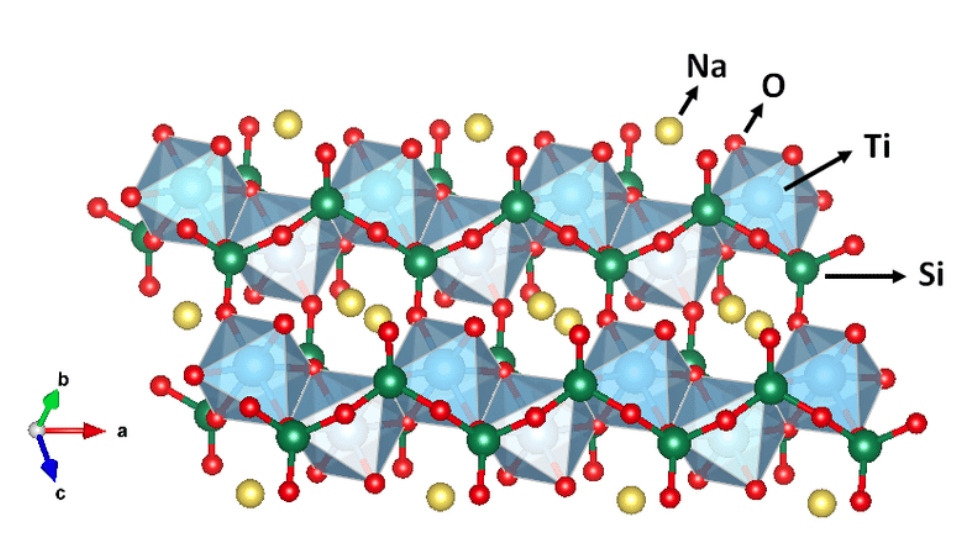
\includegraphics[scale=0.4]{NaTiSi2O6}
\caption {Структура $NaTiSi_2O_6$  ~\cite{Feiguin2019}}
\label{}
\end{figure}

Цепочки соединены между собой через вершины тетраэдров $SiO_4$. При комнатной температуре в структуре $NaTiSi_2O_6$ присутствует только одна позиция титана. Тем самым, вдоль оси $c$ образуются однородные антиферромагнитные цепочки полуцелочисленных спинов.

Величина $\chi_m$ резко убывает практически до нуля ниже 210К и не меняется при низких температурах. Остаточная восприимчивость по величине сопоставима с вкладом Ван Флека, наблюдающегося в других спин-щелевых системах в основном состоянии: $NaV_2O_5, MgV_2O_5, CaV_2O_5, CsV_2O_5$. Тем самым, основное состояние в $NaTiSi_2O_6$ может быть описано спиновым синглетом с щелью $\Delta \sim 500K$. Эта оценка была сделана исходя из аппроксимации низкотемпературной части магнитной восприимчивости по формуле $\chi_m \sim e^{\frac{-\Delta}{k_BT}}$

Структурный фазовый переход $NaTiSi_2O_6$ связан с орбитальным упорядочением. В структуре соединения магнитоактивный $Ti^{3+}$ в искаженном октаэдрическом окружении обладает двумя вырожденными $t_{2g}$ орбиталями, на которых расположен один электрон, обеспечивающий магнитное взаимодействие вдоль цепочки с участием обоих орбиталей. Ниже $T_S = 210K$ система испытывает структурный фазовый переход, который снимает вырождение $t_{2g}$ орбиталей таким образом, что при низких температурах электрон занимает наиболее низко расположенную по энергии орбиталь $d_{xy}$. Это переход приводит к сильному альтернированнию обменных взаимодействий в цепочке. В случае перекрытия орбиталей $d_{xy}$ в цепочке появляются димеры. Переход в синглетное состояние приводит к резкому уменьшению магнитной восприимчивочти при $T_S$ ~\cite{nm}.



\section{Спиновые лестницы}
В особый класс выделяют системы взаимодействующих антриферромагнитных цепочек - фазовые лестницы.

\subsection{Спиновые лестницы с нечетным числом направляющих: спиновая жидкость без щели в спектре спиновых возбуждений}
Самый простой пример спиновой лестницы с четным числом направляющих представляет собой лестница с двумя направляющими, сформированная гейзенберговскими ионами со спином $S=1/2$. Гамильтониан такой лестницы с антиферромагнитыми взаимодействиями вдоль направляющих $J$ и $J'$ ~\cite{barnes1993}:

$\hat H = J \sum\limits_{a=1,2}\sum\limits_i \hat S_{i,a} \hat S_{i+1, a} + J' \sum\limits_i \hat S_{i,1} \hat S_{i,2}$

Соотношение обменных интегралов $J$ и $J'$ является важным для формирования основного состояния, поскольку влияет на закон дисперсии и величину щели, которая разделяет основное немагнитное и первое возбужденное состояние.

Соединения $Sr_{n-1}Cu_{n+1}O_{2n}$ после обработки давление 6ГПа кристаллизуются в орторомбических структурах с пространственной группой $ Cmmm $ ~\cite{hiroi1991}.

\begin{figure}[htp]
\centering
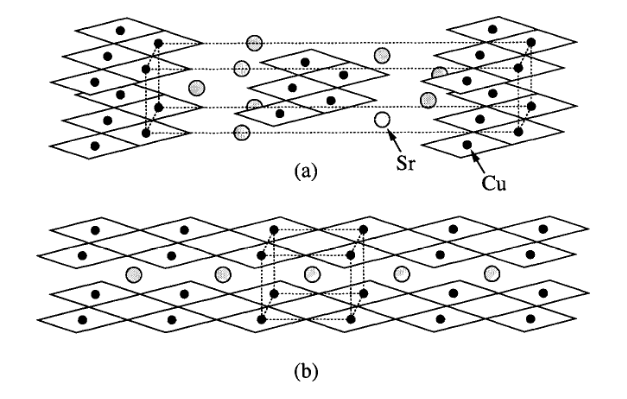
\includegraphics[scale=0.5]{SrCuO2}
\caption{Структуры кристаллов $SrCuO_2$ ($a$) - форма при низком давлении ($b$) - форма после высокого давления ~\cite{hiroi1991}}
\label{}
\end{figure}

\subsection{Зарядовый механизм димеризации спиновой лестницы}

\subsubsection{$(Sr,La,Ca)_{14}Cu_{24}O_{41}$}
Синтез и магнонные термопереносные свойства микроструктур спиновой лестницы описаны в ~\cite{adfm_202001637}, ESR (электрон спин резонанс) был изучен в ~\cite{kataev2002}

\begin{figure}[htp]
\centering
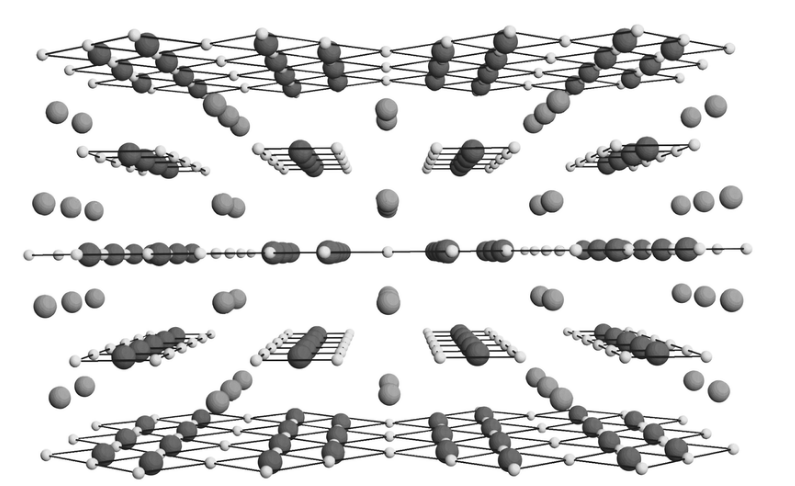
\includegraphics[scale=0.5]{Sr_14_Cu_24_O_41_a}
\caption{Структура $(Sr,La,Ca)_{14}Cu_{24}O_{41}$ ~\cite{ishii2010}}
\label{}
\end{figure}


\begin{figure}[htp]
\centering
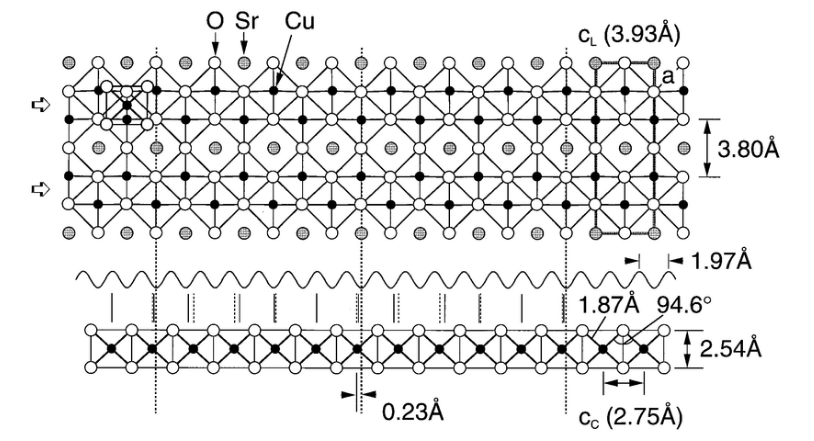
\includegraphics[scale=0.5]{Sr_14_Cu_24_O_41_b}
\caption{Схематическое изображение двух строительных блоков, двунаправленной лестничной плоскости $Cu_2O_3$ и цепочки $CuO_ 2$, в идеальном $Sr{14}Cu_{24}O_{41}$.  Цепочка $CuO_2$ расположена над серединой зигзагообразной цепочки $Cu$ в плоскости лестницы, отмеченной стрелками, а другая плоскость $Cu_2O_3$, смещенная на c $L/2$ вдоль оси c относительно первой, расположена так, чтобы для размещения цепочки $CuO_2$. Несоответствие между длинами оси c двух блоков приводит к одномерной надстройке с периодом 7c L 10c C. Синусоидальная волна, протянутая между лестницей и цепью, представляет собой потенциал несоответствия с периодом c L / 2. Вертикальные сплошные и пунктирные столбцы ниже показывают положения атомов Cu в цепочке с модификациями потенциалом несоответствия и без них, соответственно.~\cite{hiroi1996}}
\label{}
\end{figure}

\subsection{Комбинации спиновых цепочек и спиновых лестниц}

\subsection{Каркасные структуры}
Вещества относящиеся к семейству ванадиевых бронз $\beta{\beta'}-$ типа с общей формулой $\beta{\beta'}-A_xV_2O_5$ где $A=Li, Cs, Ca, Mg, Na, Sr, Cu$ и т.д., являются квазиодномерными проводниками ~\cite{Ueda_1998}. Однии из представителей этого семейства является квазиодномерное соединение с переменной валентностью $\beta-Na_{0,33}V_2O_5$, в котором при понижении температуры наблюдается несколько фазовых переходов типа порядок-беспорядок, каждый из которых связан с упорядочением одной из подсистем $\beta-Na_{0,33}V_2O_5$ ~\cite{nm}. Вещество последовательно испытывает структурный ($T_s \sim 230K$), зарядовый ($T_C \sim 136K$) и магнитный ($T_N \sim 22K $) фазовые переходы ~\cite{yamada1999, yamauchi2002, onoda1982, presura2003}. 

Ниже приведены данные из проекта MaterialProject ~\footnote{~\url{https://materialsproject.org/materials/mvc-8363/}}

\begin{figure}[htp]
\centering
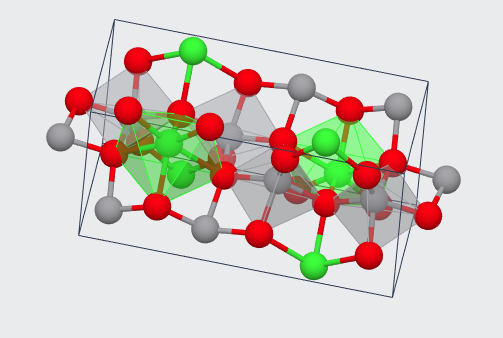
\includegraphics[scale=0.7]{CaV_2O5}
\caption{Структура $CaV_2O_5$, где $Ca$-зеленый, $O$ - красный, $V$-серый}
\label{}
\end{figure}

Моноклинная кристаллическая структура ($A2/m$) этих элементов в $\beta (\beta')$-фазе содержит вытянутые вдоль оси $b$ туннели, образованные $V-O$ комплексами. Внутри туннелей расположены ионы $Na$. При высоких температурах в $\beta-Na_{0.33}V_2O_5$ для ионов ванадия существуют три различные кристаллографические позиции ~\cite{nm}:
\begin{itemize} 
\item V1 в октаэдрическом окружении ионов кислорода формирует вдоль оси b зигзаговые цепочки из соединенных по ребру октаэдров $VO_6$
\item V2 в таком же окружении образует двойные цепочки из соединенных по углу октаэдров
\item V3 формирует зигзаговые цепочки из пирамид $VO_5$, соединенных по ребру
\end{itemize} 

В каждой элементарной ячейке существуют также две кристаллографические позиции для ионов $Na^{+}$ (в случае $NaV_2O_5$). С понижением температуры при  $T_S$ происходит структурное упорядочивание ионов $Na$, и вдоль оси $b$ возникает <<сверхструктура>> типа 1x2x1.


\section{Химические реакции получения магнетиков}
При исследовании способа производства новых магнетиков использовались реакции в формате CML, извлеченные путем интеллектуального анализа текста из патентов США ~\footnote{\url{https://www.google.com/googlebooks/uspto-patents.html}}, опубликованных с 1976 по сентябрь 2016 года. 

Реакции были извлечены с использованием ~\cite{extraction_cml, extraction_cml_1, extraction_cml_2, extraction_cml_3}, с помощью ПО LeadMine ~\footnote{\url{https://www.nextmovesoftware.com/leadmine.html}}, используемого для распознавания химических символов.

\subsection{$Rb_4Cu(MoO_4)_3$}
Синтез производится флюс методом и детально описан в ~\cite{lsu}

\subsection{$VO(CH_3COO)_2$}
Синтез $VO(CH_3COO)_2$ подробно описан в ~\cite{paul2007} и основан на следующих постулатах:

\begin{itemize} 
\item $V_2O_5+2(CH_3CO)_2O \rightarrow 2VO(CH_3COO)_2+\frac{1}{2}O_2$
\item $V_2O_5+3(CH_3CO)_2O \rightarrow 2[VO(CH_3COO)_3]$ \\
$2[VO(CH_3COO)_3] \rightarrow 2VO(CH_3COO)_2 + 2[CH_3COO]$ \\
$2[CH_3COO] \rightarrow CH_3 \cdot CH_3 +2CO_2 $ \\
\end{itemize} 


\subsection{$\gamma-Li_2CuZrO_4$}
В ~\cite{dussarrat2002} приводится синтез двух полиморфов $Li_2CuZrO_4$ путем твердофазной  реакцией $Li_2CO_3$, $ZrO_2$ и $CuO$ в интервале температур 700 - 1100° C.

\subsection{$LiCu_2O_2$}
Кристаллы $LiCu_2O_2$, выращивают спонтанной кристаллизацией из флюсованного расплава ~\cite{paszkowicz2001}.


\subsection{$NaCu_2O_2$}
Аналогично $LiCu_2O_2$

\subsection{$RbCuAl(PO_4)_2$}
$RbCuAl(PO_4)_2$ получается гидротермальным синтезом при 553К ~\cite{yakubovich2016}.

\subsection{$Sr_4Cu_6O_{10}$}
Стартовые оксиды имеющие различное отношение $Sr/Cu$ упаковываются в золотоую капсулу и сжимаются давлением 6ГПа с нагревом до $1273 \sim 1573$K на полчаса.


\subsection{$NaV_2O_5$}
В марте 2015 был опубликован новый метод ~\cite{acsami_5b01260} \\

Предшествующие методы: \\

- твердотельная реакция ~\cite{raistrick1983} \\

- метод флюса ~\cite{rabia2009} \\

- метод золь-гель ~\cite{pereira_ramos1988, bach1990} \\

- гидротермальный метод ~\cite{xu2011} \\

\subsection{$CaV_2O_5$}
Твердотельная реакция по аналогии с $NaV_2O_5$

\subsection{$MgV_2O_5$}
В качестве активного материала используют коммерческий $V_2O_5$ (Sigma Aldrich, 99,6\%) с микрометрическим размером частиц. $MgV_2O_5$ был синтезирован двумя способами ~\cite{verrelli2018}: \\

- твердофазной реакции между $MgO$ и $VO_2$ ~\cite{bouloux1976}. Стехиометрическую порошковую смесь предварительно нагретого (500 ° C, 2 ч) MgO и VO2 отжигали в течение 6 ч при 900 ° C. $VO_2$ был получен путем пропорционального разделения $V_2O_5$ и $V_2O_3$. Стехиометрические количества порошков $V_2O_3$ и $V_2O_5$ смешивали и измельчали вместе, а затем отжигали при 650 ° C в течение 10 ч в вакууме. В качестве держателей образцов использовали листы платины, прокатанные в тигле из $Al_2O_3$. Предшественник $V_2O_3$ был приготовлен восстановлением $V_2O_5$ в потоке чистого $H_2$ (100 мл / мин), генерируемого электролизом воды. Применяли две последовательные стадии отжига по 2 часа при 500 и 700 ° C, и образец дополнительно охлаждали естественным образом в потоке газа $H_2$ в течение примерно 10 часов.\\

- компропорционирования $MgV_2O_4$ и $MgV_2O_6$. Стехиометрические количества $MgV_2O_6$ и $MgV_2O_4$ измельчали вместе и отжигали при 770 ° C в течение 12 ч в вакууме. Предшественник $MgV_2O_6$ был приготовлен путем смешивания $V_2O_5$ с источником $Mg^{2+}$, таким как $MgO$, $Mg(OH)_2$ или $4MgCO_3 · Mg (OH)_2 · 5H_2O$ (независимо от используемого источника $Mg$ был получен тот же продукт). Смесь прекурсоров, помещенных в листы $Pt$, прокатанные в $Al_2O_3$ тигле, прокаливали в течение 15 ч при 650 ° C на воздухе. $MgV_2O_4$ был получен восстановлением $MgV_2O_6$ в газовой среде $H_2$ при 700 ° C в течение 4 ч.

Приготовление твердых растворов $Mg_xV_2O_5$ (x = 0,7 и 0,9) было предпринято путем твердофазной реакции порошков $MgV_2O_5$ и $V_2O_5$ (смешанное молярное соотношение в x: (1-x)) или, иначе, путем взаимодействия $MgO$, $VO_2$ и $V_2O_5$ в x: 2x: (1-x) молярное соотношение. В обоих случаях смешанные прекурсоры отжигались при 900 ° C в течение 6 ч в вакууме. Все это привело к смесям в основном $MgV_2O_5$ и $VO_2$ и поэтому не будет обсуждаться далее. Альтернативные попытки получить $Mg_xV_2O_5$ ($x \le 1$) путем химического восстановления $V_2O_5$ с помощью $MgI_2$ (с использованием молярных соотношений $V_2O_5$: $MgI_2$ 1: 0,5 и 1: 1) также потерпели неудачу. $CaV_2O_5$ был получен реакцией компропорционирования из $CaV_2O_4$ и $CaV_2O_6$. Повторный отжиг прекурсоров смешанного порошка проводили в вакууме при 650 ° C (два шага по 10 часов), 750 ° C (12 часов) и 800 ° C (два шага по 12 часов). Листы $Pt$, прокатанные в тиглях из $Al_2O_3$, использовались в качестве держателей образцов, за исключением последней стадии отжига, на которой применялся тигель из $Мо$. $CaV_2O_6$ был получен твердофазной реакцией между $CaCO_3$ и $V_2O_5$ (650 ° C, 12 ч, атмосферный воздух), тогда как $CaV_2O_4$ был получен восстановлением $CaV_2O_6$ под газом $H_2$ при 700 ° C в течение 4 часов. Попытки химического окисления порошков $MgV_2O_5$ и $CaV_2O_5$ были предприняты реакцией с $NO_2BF_4$ (молярное превышение 100\%) при 80° C в ACN в течение 6 и 24 ч при непрерывном барботировании $Ar$. После завершения реакции образцы промывали dryACN, фильтровали под вакуумом.

\begin{figure}[htp]
\centering
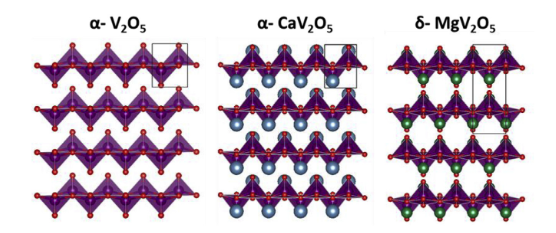
\includegraphics[scale=0.7]{V_2O_5}
\caption{ Кристаллическая структура первичных полиморфов $\alpha-V2O5$, $\alpha-CaV2O5$ на плоскости $b-c$ и полиморфа $\delta-MgV2O5$ на плоскости $a-b$. ~\cite{verrelli2018}}
\label{}
\end{figure}

\subsection{$CsV_2O_5$}
В ~\cite{luo2013} $CsV_2O_5$ c пространственной группой симметрии $P_{21/c}$ был синтезирован твердофазной реакцией.

До этого синтезировали двумя методами (с одним недостатком - получалась центросимметричная структура и не имела откликов генерации второй гармоники (ГВГ)): \\

- электролиз расплава $Cs_2O$ и $V_2O_5$ при высокой температуре ~\cite{mumme_1971}, \\

- твердофазная реакция смесей с соответствующими мольными соотношениями $CsVO_3$, $V_2O_3$ и $V_2O_5$ в вакуумированной кремнеземной трубке ~\cite{Ueda_1998}

Коричневые монокристаллы $CsV_2O_5$ получены высокотемпературной твердотельной реакцией. Стехиометрические количества $Cs_2CO_3$ (AR) и $V_2O_5$ (AR) были точно взвешены. Эти смеси прессовали в таблетки и затем помещали в платиновый тигель. Была выбрана платина, поскольку она химически инертна в этой системе. Образцы постепенно нагревали до 500 ° C в течение 15 ч, выдерживали в течение 120 ч, а затем позволяли остыть примерно до 100 ° C при контролируемой скорости снижения температуры 10 ° C / ч в печи в атмосфере монооксида углерода. Изоморфные фазы $AV_2O_5$ (A = Na, K, Rb) не были получены тем же методом.

\begin{figure}[htp]
\centering
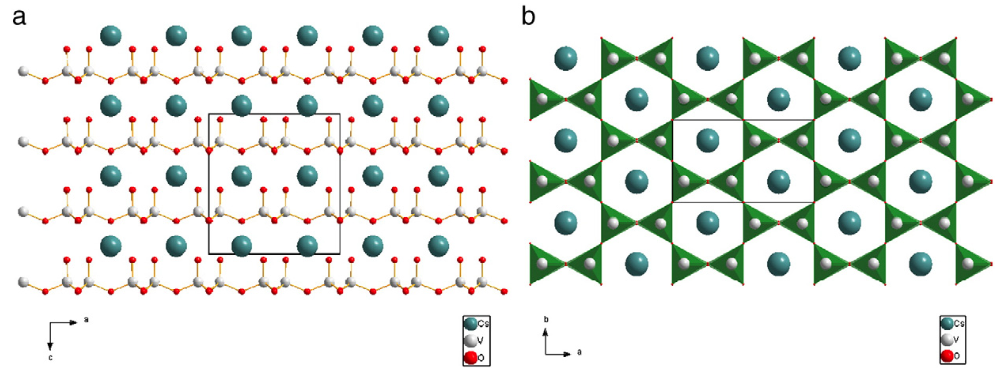
\includegraphics[scale=0.35]{CsV_2O_5}
\caption{Кристаллическая решетка $CsV_2O_5$ ~\cite{luo2013}}
\label{}
\end{figure}


\subsection{$SrNi_2V_2O_8$}
В {vogt1990} описано получение $SrNi_2V_2O_8$ и $BaCu_2V_2O_8$ химическими реакциями в твердом состоянии ниже точки плавления из реакционной смеси $BaCO_3$, $CuO$, $V_2O_5$ Изолированные темно-красные монокристаллы приводят к тетрагональной симметрии: пространственная группа $D_{2d}^{12}-I42d$, $a = 12.744$; $с = 8,148$A ; $Z = 8$. Кристаллическая структура тесно связана с типом $SrNi_2V_2O_8$. Основная разница связана с координацией меди кислородом.
Также, на рынке представлен ксерогель $V_2O_5 \cdot nH_2O$ - является основой для синтеза нанотрубок оксида ванадия 250 руб./г.


\subsection{$(Sr,La,Ca)_{14}Cu_{24}O_{41}$}
Исходя из публикации ~\cite{khan_afzal_2011_dA_finitif} производство требует промышленного оборудования, возможно, что химической лаборатории будет недостаточно. Синтез основан на равновесии системы $SrO-CuO$ для которого построена фазовая диаграмма

\begin{figure}[htp]
\centering
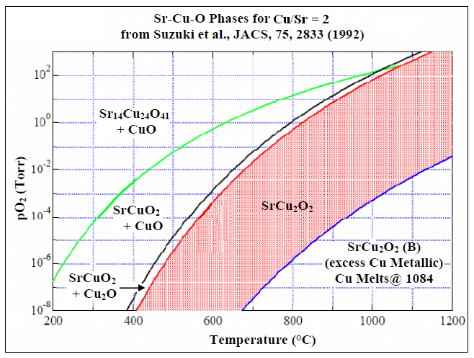
\includegraphics[scale=0.9]{Sr_14_Cu_24_O_41_ph}
\caption{Фазовая диаграмма системы Sr-Cu-O. Зависимость от парциального давления $O_2$ и температуры.~\cite{hiroi1996}}
\label{}
\end{figure}

Используется метод CVD - это химический процесс, используемый для получения высокочистых и высокоэффективных твердотельных материалов. Этот процесс часто используется в полупроводниковой промышленности для производстве тонких пленок ~\cite{cvd}
CVD - это процесс осаждения, при котором химические прекурсоры транспортируется в паровой фазе для разложения на предварительно нагретой подложке с образованием тонкой пленки ~\cite{cvd_1}.

\begin{figure}[htp]
\centering
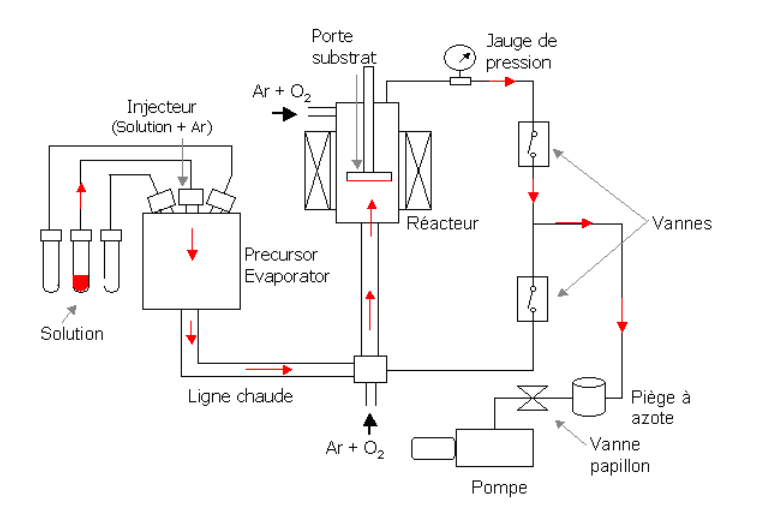
\includegraphics[scale=0.6]{mocvd}
\caption{Схема лабораторной установки по производству  $Sr_{14}Cu_{24}O_{41}$ методом MOCVD ~\cite{khan_afzal_2011_dA_finitif}}
\label{}
\end{figure}

Оксид стронция получают прокаливанием карбоната стронция при темературе около $1400^\circ $


\subsection{$LiCu_2O_2$}
\begin{tabular}{|l|l|l|}
\hline
	Наименование  & Производитель & Цена, руб./г\\
\hline
	$Металлический порошок лития$ & СтальЭнерго-96 & 2,5\\
\hline	
	Итого & & 2,5 \\
\hline
\end{tabular}


\subsection{$\beta-Na_{0.33}V_2O_5$}

\begin{tabular}{|l|l|l|}
\hline
	Наименование  & Производитель & Цена, руб./г\\
\hline
	$NaX$ & - &  - \\
\hline
	$V_2O_5$ & РСТД & 9,5\\
\hline	
	Итого & & 9,5 \\
\hline
\end{tabular}

\subsection{$CuAl(AsO_4)O$}
Минерал урусовит - можно купить в естественном виде.


\subsection{$Cu(CF_3COO)_2$}
В ~\cite{rsc_c_2012} трифторацетат меди(II) был получен, методом ~\cite{Polyhedron_18_22}, реакцией основного карбоната меди(II) $CuCO_3$ (аналитическая марка, POCh, Польша) с трифторуксусной кислотой (99\%, Aldrich) $CF_3COOH$ в водно–этанольном растворе.


\section{Экономическая оценка постановки экспериментов}
Экономическая оценка стоимости экспериментов будет складываться из стоимости компонентов реакций, с выходом продукта достаточным для производства мишений для дальнейшего облучения их ионизационным излучением. Считается, что химическая лаборатория есть и вложений в лабораторное оборудование не требуется. Цены взяты из интернет на ноябрь 2020г.

\subsection{$Rb_4Cu(MoO_4)_3$}
\begin{tabular}{|l|l|l|}
\hline
	Наименование  & Производитель & Цена, руб./г\\
\hline
	Рубидий иодид ХЧ & Югреактив & 0,158  \\
\hline
	Молибден - проволока & АвиаПромСталь & 1,16\\
\hline	
	Итого & & 1,318 \\
\hline
\end{tabular}


\subsection{$VO(CH_3COO)_2$}
\begin{tabular}{|l|l|l|}
\hline
	Наименование  & Производитель & Цена, руб./г\\
\hline
	$(CH_3CO)_2O$ & Химпромкомплект & 0,001  \\
\hline
	$V_2O_5$ & РСТД & 0,65\\
\hline	
	Итого & & 0,651 \\
\hline
\end{tabular}



\subsection{$CsV_2O_5$}
\begin{tabular}{|l|l|l|}
\hline
	Наименование  & Производитель & Цена, руб./г\\
\hline
	$Cs_2CO_3$ & ochv.ru &  15 \\
\hline
	$V_2O_5$ & РСТД & 9,5\\
\hline	
	Итого & & 14,5 \\
\hline
\end{tabular}

\subsection{$Sr_4Cu_6O_{10}$}
\begin{tabular}{|l|l|l|}
\hline
	Наименование  & Производитель & Цена, руб./г\\
\hline	
	оксид $Sr$ & МХК & 0.48\\
\hline	
	оксид $Cu$ & pcgroup.ru & 1.75\\
\hline	
	Итого & & 2,23 \\

\hline
\end{tabular}


\subsection{$SrNi_2V_2O_8$}
\begin{tabular}{|l|l|l|}
\hline
	Наименование  & Производитель & Цена, руб./г\\
\hline
	$SrСO_3$ & Профснаб &  0,798 \\
\hline
	$NiO$ & Профснаб & 1,310 \\
\hline
	$V_2O_5$ & РСТД & 9,5\\
\hline	
	Итого & & 11,608 \\
\hline
\end{tabular}

\subsection{$BaCu_2V_2O_8$}
\begin{tabular}{|l|l|l|}
\hline
	Наименование  & Производитель & Цена, руб./г\\
\hline
	$BaCO_3$ & Профснаб & 0,378 \\
\hline
	$CuO$ & Профснаб & 0,905 \\
\hline
	$V_2O_5$ & РСТД & 9,5\\
\hline	
	Итого & & 10,783 \\
\hline
\end{tabular}


\subsection{$(Sr,La,Ca)_{14}Cu_{24}O_{41}$}

\begin{tabular}{|l|l|l|}
\hline
	Наименование  & Производитель & Цена, руб./г\\
\hline
	$SrСO_3$ & Профснаб &  0,798 \\
\hline
	CuO & Профснаб & 0,905 \\
\hline
	Итого & & 1.703 \\
\hline
\end{tabular}


\subsection{$Cu(CF_3COO)_2$}

\begin{tabular}{|l|l|l|}
\hline
	Наименование  & Производитель & Цена, руб./г\\
\hline
	Трифторуксусная кислота & Русский химик & 7.750 \\
\hline
	Карбонат меди & Ареолаб & 2.264\\
\hline
	Этиловый спирт & Авито & 0.3\\
\hline
	Итого & & 10.314 \\
\hline
\end{tabular}

\subsection{$\beta-Na_{0.33}V_2O_5$}

\begin{tabular}{|l|l|l|}
\hline
	Наименование  & Производитель & Цена руб./г\\
\hline
	Ванадий (ВнП-1) & Метотехника & 50 \\
\hline
	Натрий сернистый & Русский химик & 0.587\\
\hline
	Сера & Русский химик & 0,173 \\
\hline
	$Al_2O_3$ & Металлопторг & 0,150 \\	
\hline
	Итого & & 50,91\\
\hline
\end{tabular}	

\section{Заключение}
В работе были рассмотрены новые магнетики с одномерной кристаллической структурой, их основные свойства и способы синтеза. Данные материалы ранее подвергались излучению с целью изучения кристаллической решетки, зачастую это было рентгеновское излучение, но иногда, например в ~\cite{dussarrat2002} рентгеновское, нейтронная и электронная дифракция, но не изучалось комплексное влияние ионизирующего излучения на их свойства. 

Видится перспективным провести исследования для выше описанных низкоразмерных магнетиков по измерению:

\begin{itemize} 
\item полного сечения
\item спектра рассеяния
\item магнитной восприимчивости
\item проводимости
\item теплоемкости
\item изменения параметров фазовых переходов
\end{itemize} 

под воздействием:
\begin{itemize} 
\item $\alpha$
\item $\beta$
\item $\gamma$
\item нейтронного излучения
\item электрононы или мюоны
\end{itemize} 

по трем направлениям кристаллографических осей
\begin{itemize} 
\item $a(x)$
\item $b(y)$
\item $c(z)$
\end{itemize} 

с целью исследования возможности построения квантового компьютера на ионизирующем излучении, действующего на одном или нескольких принципах:
\begin{itemize} 
\item изменения спина и магнетизма
\item изменения проводимости
\item температурного расширения/сжатия
\end{itemize} 

Эксперименты можно будет провести на стендах описанных в предыдущей работе <<Теоретическое исследование возможности построения квантового компьютера на источниках ионизирующего излучения>> ,а результаты экспериментов можно будет верифицировать теоретическими рассчетами, приведенными в - <<Программное моделирование цепочки Гейзенберга S=1/2>>.

Предлагаю рассмотреть перспективность подачи заявки в РФФИ на получение финансирования данных иследовательских работ.

\begin{thebibliography}{3}
\bibitem{mp}
Катанин А.А., Ирхин В.Ю., Игошев П.А. // Модельные подходы к магнетизму двумерных зонных систем. -- М.:ФИЗМАТЛИТ, 2013

\bibitem{nm}
Васильев А.Н., Волкова О.С., Зверева Е.А., Маркина М.М. // Низкоразмерный магнетизм. -- М.: ФИЗМАТЛИТ, 2018
 
\bibitem{cml}
Peter Murray-Rust and Henry S. Rzepa // Chemical Markup, XML, and the Worldwide Web. 1. Basic Principles -- Virtual School of Molecular Sciences, School of Pharmaceutical Sciences, University of Nottingham, U.K.,and Department of Chemistry, Imperial College of Science, Technology and Medicine,London SW72AY, U.K ~\url{https://doi.org/10.1021/ci990052b}, 1999

\bibitem{extraction_cml}
Lowe, Daniel Mark // Extraction of chemical structures and reactions from the literature -- University of Cambridge,  ~\url{https://doi.org/10.17863/CAM.16293}, 2012

\bibitem{extraction_cml_1}
David M. Jessop, Sam Adams, Peter Murray-Rust // Mining chemical information from Open patents -- Murray-Rust group, Unilever Centre for Molecular Science Informatics, Department of Chemistry, University of Cambridge, ~\url{https://core.ac.uk/reader/1334263}, 2011

\bibitem{extraction_cml_2}
D.M.Jessop // Information extraction from chemical patents -- Organisation for Economic Co-Operation and Development (OECD), ~\url{http://www.dspace.cam.ac.uk/handle/1810/238302}, 2011

\bibitem{extraction_cml_3}
David M. Jessop, Sam E. Adams, Egon L. Willighagen, Lezan Hawizy and Peter Murray-Rust // OSCAR4: a flexible architecture for chemical text-mining -- ~\url{http://www.dspace.cam.ac.uk/handle/1810/239919}, 2011

\bibitem{Polyhedron_18_22}
E.Szłyk, I.Szymańska // Studies of new volatile copper(I) complexes with triphenylphosphite and perfluorinated carboxylates -- Polyhedron, Volume 18, Issue 22, DOI: ~\url{https://doi.org/10.1016/S0277-5387(99)00199-0}, 24 September 1999, Pages 2941-2948

\bibitem{rsc_c_2012}
Robert Szczęsny, Edward Szłyk,b Marek A. Wiśniewski, Tuan K. A. Hoang,a Duncan H. Gregory // Facile preparation of copper nitride powders and nanostructured films -- Royal Society of chemystry, Accepted Manuscript, 2012 -- ~\url{https://pubs.rsc.org/fi/content/getauthorversionpdf/C6TC00493H}

\bibitem{acsami_5b01260}
Jae-Kwang Kim, B. Senthilkumar, Sun Hye Sahgong, Jung-Hyun Kim, Miaofang Chi, and Youngsik Kim
ACS Applied Materials \& Interfaces 2015 7 (12), 7025-7032, DOI: ~\url{https://doi.org/10.1021/acsami.5b01260}

\bibitem{raistrick1983}
D.Raistrick \\ Lithium insertion reactions in tungsten and vanadium oxide bronzes -- Solid State Ionics, Volumes 9–10, Part 1, December 1983, Pages 425-430, DOI: ~\url{https://doi.org/10.1016/0167-2738(83)90270-9}

\bibitem{rabia2009}
K. Rabia, A. Pashkin, S. Frank, G. Obermeier, S. Horn, M. Hanfland and C. A. Kuntscher (2009) // High-pressure XRD study of $\beta-Na_{0.33}V_2O_5$, High Pressure Research, 29:4, 504-508, DOI: ~\url{https://doi.org/10.1080/08957950903422436}

\bibitem{pereira_ramos1988}
J.P.Pereira-Ramos, R.Messina, L.ZnaidiN.Baffier // Electrochemical lithium intercalation in $Na_{0.33}V_2O_5$ bronze prepared by sol-gel processes -- Solid State Ionics, Volumes 28–30, Part 1, September 1988, Pages 886-894, DOI: ~\url{https://doi.org/10.1016/S0167-2738(88)80164-4}

\bibitem{bach1990}
S.Bach,J.P.Pereira-Ramos, N. Baffier and R. Messina// A Thermodynamic and Kinetic Study of Electrochemical Lithium Intercalation in $Na_{0.33}V_2O_5$ Bronze Prepared by a Sol-Gel Process -- Journal of The Electrochemical Society, Volume 137, Number 4, ~\url{https://doi.org/10.1149/1.2086601}

\bibitem{xu2011}
Xu, Yang and Han, Xiaosan and Zheng, Lei and Yan, Wensheng and Xie, Yi // Pillar effect on cyclability enhancement for aqueous lithium ion batteries: a new material of $\beta - $ vanadium bronze $M_{0.33}V_2O_5$ (M = Ag,Na) nanowires -- J. Mater. Chem. 2011, 21, 14466–14472, DOI: ~\url{https://doi.org/10.1039/C1JM11910A}

\bibitem{kataev2002}
Kataev, V. and Choi, Kwangyong and Grüninger, Markus and Ammerahl, U. and Büchner, Bernd and Freimuth, A. and Revcolevschi, Alex // ESR study of $(Sr,La,Ca)_{14}Cu_{24}O_{41}$ -- Physica B: Condensed Matter Volumes 312–313, March 2002, Pages 614-616,  ~\url{https://doi.org/10.1016/S0921-4526(01)01288-1}

\bibitem{hiroi1996}
Z.Hiroi, S.Amelinckx and G.Van Tendeloo, N.Kobayashi // Microscopic origin of dimerization in the $CuO_2$ chains in $Sr_{14}Cu_{24}O_{41}$ -- January 1997, Physical review. B, Condensed matter 54(22):15849-15855, DOI: ~\url{https://doi.org/10.1103/PhysRevB.54.15849} 

\bibitem{adfm_202001637}
Chen, X., Kim, J., Jia, Q., Sullivan, S. E., Xu, Y., Jarvis, K., … Shi, L. (2020). Synthesis and Magnon Thermal Transport Properties of Spin Ladder Sr 14 Cu 24 O 41 Microstructures. Advanced Functional Materials, 2001637, DOI: ~\url{https://doi.org/10.1002/adfm.202001637}

\bibitem{khan_afzal_2011_dA_finitif}
Afzal Khan. Synthesis of Strontium Cuprate (SrCu2O2) by MOCVD as a P-type Transparent Con-ducting Oxide Thin Film.. Condensed Matter [cond-mat]. Institut National Polytechnique de Greno-ble - INPG; Université de Grenoble, 2011. English.

\bibitem{cvd}
Chemical vapor deposition -- ~\url{ http://en.wikipedia.org/wiki/chemical_vapor_deposition}

\bibitem{cvd_1}
A.R.Barron // Chemical   vapor   deposition.Technical   report, ~\url{http://cnx.org/content/m25495/1.2/} -- 2009

\bibitem{vogt1990}
Vogt, R., and Muller-Buschbaum, H. (1990). $BaCu_2V_2O_8$: Eine Variante des $SrNi_2V_2O_8$-Typs, mit $Cu_2+$ in 4+1+1-Koordination. Zeitschrift Fur Anorganische Und Allgemeine Chemie, 591(1), 167–173. DOI: ~\url{https://doi.org/10.1002/zaac.19905910119}

\bibitem{luo2013}
Luo, H., Pan, J., Lou, B., Li, Y., Li, X., and Han, L. (2013). Synthesis, crystal structure and nonlinear optical property of $CsV_2O_5$. Inorganic Chemistry Communications, 27, 79-81. DOI: ~\url{https://doi.org/10.1016/j.inoche.2012.10.023} 

\bibitem{mumme_1971}
W.G. Mumme, J.A. Watts, The crystal structure of reduced cesium vanadate,$CsV_2O_5$, J. Solid State Chem. 3 (1971) 319–322

\bibitem{Ueda_1998}
Y. Ueda, M. Isobe Magnetic, Properties of $AV_20_5$(A = Li, Na, Cs, Ca and Mg) Journal of Magn, Magn. Mater. 177–181 (1998) 741–742.

\bibitem{Ueda_2002}
Y. Ueda, M. Isobe, T.Yamauchi // Journal of Physics and Chemistry of Solids, 2002, V.63, p.951


\bibitem{verrelli2018}
Verrelli, R., Black, A. P., Pattanathummasid, C., Tchitchekova, D. S., Ponrouch, A., Oró-Solé, J., … Palacín, M. R. (2018). On the strange case of divalent ions intercalation in $V_2O_5$. Journal of Power Sources. doi: ~\url{https://doi.org/10.1016/j.jpowsour.2018.08.024} 

\bibitem{bouloux1976}
Bouloux, J.-C., Milosevic, I., and Galy, J. (1976). Les hypovanadates de magnésium MgVO3 et $MgV_2O_5$. Structure cristalline de $MgVO_3$. Journal of Solid State Chemistry, 16(3-4), 393–398. doi:~\url{https://doi.org/10.1016/0022-4596(76)90056-6} 

\bibitem{ishii2010}
Ishii, R., Gautreaux, D., Onuma, K., Machida, Y., Maeno, Y., Nakatsuji, S., and Chan, J. Y. (2010). Low-Dimensional Structure and Magnetism of the Quantum Antiferromagnet $Rb_4Cu(MoO_4)_3$ and the Structure of $Rb_4Zn(MoO_4)_3$. Journal of the American Chemical Society, 132(20), 7055–7061. doi:~\url{https://doi.org/10.1021/ja100077v }

\bibitem{yamada1999}
Yamada, H., and Ueda, Y. (1999). Magnetic, Electric and Structural Properties of $\beta-A_xV_2O_5(A=Na, Ag)$. Journal of the Physical Society of Japan, 68(8), 2735–2740. doi:~\url{https://doi.org/10.1143/jpsj.68.2735}                                                                                                                                                                                                                                                                                                                                                                                                                                                                                                                                                                                                                                                                                                                                                                                                                                                                                                                                                                                                                                                                                                                                                                                                                                                                                                                                                                                                                                                                                                                                                                                                                                                                                                                                                                                                                                                                                                                                                                                                                                                                                                                                                                                                                                                                                                                                                                                                                                                                                                                                                                                                                                                                                                                                                                                                                                                                                                                                                                                                                                                                                                                                                                                                                                                                                                                                                                                                                                                                                                                                                                                                                                                                                                                                                                                                                                                                                                                                                                                                                                                                                                                                                                                                                                                                                                                                                                                                                                                                                                                                                                                                                                                                                                                                                                                                                                                                                                                                                                                                                                                                                                                                                                                                                                                                                                                                                                                                                                                                                                                                                                                                                                                                                                                                                                                                                                                                                                                                                                                                                                                                                                                                                                                                                                                                                                                                                                                                                                                                                                                                                                                                                                                                                                                                                                                                                                                                                                                                                                                                                                                                                                                                                                                                                                                                                                                                                                                                                                                                                                                                                                                                                                                                                                                                                                                                                                                                                                                                                                                                                                                                                                                                                                                                                                                                                                                                                                                                                                                                                                                                                                                                                                                                                                                                                                                                                                                                                                                                                                                                                                                                                                                                                                                                                                                                                                                                                                                                                                                                                                                                                                                                                                                                                                                                                                                                                                                                                                                                                                                                                                                                                                                                                                                                                                                                                                                                                                                                                                                                                                                                                                                                                                                                                                                                                                                                                                                                                                                                                                                                                                                                                                                                                                                                                                                                                                                                                                                                                                                                                                                                                                                                                                                                                                                                                                                                                                                                                                                                                                                                                                                                                                                                                                                                                                                                                                                                                                                                                                                                                                                                                                                                                                                                                                                                                                                                                                                                                                                                                                                                                                                                                                                                                                                                                                                                                                                                                                                                                                                                                                                                                                                                                                                                                                                                                                                                                                                                                                                                                                                                                                                                                                                                                                                                                                                                                                                                                                                                                                                                                                                                                                                                                                                                                                                                                                                                                                                                                                                                                                                                                                                                                                                                                                                                                                                                                                                                                                                                                                                                                                                                                                                                                                                                                                                                                                                                                                                                                                                                                                                                                                                                                                                                                                                                                                                                                                                                                                                                                                                                                                                                                                                                                                                                                                                                                                                                                                                                                                                                                                                                                                                                                                                                                                                                                                                                                                                                                                                                                                                                                                                                                                                                                                                                                                                                                                                                                                                                                                                                                                                                                                                                                                                                                                                                                                                                                                                                                                                                                                                                                                                                                                                                                                                                                                                                                                                                                                                                                                                                                                                                                                                                                                                                                                                                                                                                                                                                                                                                                                                                                                                                                                                                                                                                                                                                                                                                                                                                                                                                                                                                                                                                                                                                                                                                                                                                                                                                                                                                                                                                                                                                                                                                                                                                                                                                                                                                                                                                                                                                                                                                                                                                                                                                                                                                                                                                                                                                                                                                                                                                                                                                                                                                                                                                                                                                                                                                                                                                                                                                                                                                                                                                                                                                                                                                                                                                                                                                                                                                                                                                                                                                                                                                                                                                                                                                                                                                                                                                                                                                                                                                                                                                                                                                                                                                                                                                                                                                                                                                                                                                                                                                                                                                                                                                                                                                                                                                                                                                                                                                                                                                                                                                                                                                                                                                                                                                                                                                                                                                                                                                                                                                                                                                                                                                                                                                                                                                                                                                                                                                                                                                                                                                                                                                                                                                                                                                                                                                                                                                                                                                                                                                                                                                                                                                                                                                                                                                                                                                                                                                                                                                                                                                                                                                                                                                                                                                                                                                                                                        

\bibitem{yamauchi2002}
Yamauchi, T., Ueda, Y., and Môri, N. (2002). Pressure-Induced Superconductivity in $\beta−Na_{0.33}V_2O_5$ beyond Charge Ordering. Physical Review Letters, 89(5). doi:~\url{https://doi.org/10.1103/physrevlett.89.057002} 

\bibitem{onoda1982}
Onoda, M., Takahashi, T., and Nagasawa, H. (1982). Microscopic Evidences of Bipolarons in the Quasi-One-Dimensional Conductor $\beta-Na_{0.33}V_2O_5$. Journal of the Physical Society of Japan, 51(12), 3868–3875. doi:~\url{https://doi.org/10.1143/jpsj.51.3868} 

\bibitem{presura2003}
Presura, C., Popinciuc, M., van Loosdrecht, P. H. M., van der Marel, D., Mostovoy, M., Yamauchi, T., and Ueda, Y. (2003). Charge-Ordering Signatures in the Optical Properties of $\beta-Na_{0.33}V_2O_5$. Physical Review Letters, 90(2). doi:~\url{https://doi.org/10.1103/physrevlett.90.026402} 

\bibitem{weeks2003}
Weeks, C., Song, Y., Suzuki, M., Chernova, N. A., Zavalij, P. Y., and Whittingham, M. S. (2003). The one dimensional chain structures of vanadyl glycolate and vanadyl acetateElectronic supplementary information (ESI) available: difference plots and reflections lists for $ VO(CH_3COO)_2 $ and $VO(OCH_2CH_2O)$. Journal of Materials Chemistry, 13(6), 1420. doi:~\url{https://doi.org/10.1039/b208100h}

\bibitem{koo2010}
Koo, H.-J., and Whangbo, M.-H. (2010). Spin dimer and mapping analyses of the magnetic properties of $VO(CH_3CO_2)_2$ and $VO(OCH_2CH_2O)$. Solid State Sciences, 12(5), 685–690. doi:~\url{https://doi.org/10.1016/j.solidstatesciences.2009.03.023} 

\bibitem{lsu}
Gautreaux, Dixie Plaisance, <<Investigation of Antimonide Structure Types and the Structural Studies of Molybdates>> (2008). LSU Doctoral Dissertations. 2617. ~\url{https://digitalcommons.lsu.edu/gradschool_dissertations/2617}

\bibitem{paul2007}
Paul, R. C., Bhatia, S., Kumar, A., Mague, J. T., and Weston, C. W. (2007). Vanadyl(IV) Acetate, VO(CH3 CO2 )2 . Inorganic Syntheses, 181–183. doi:~\url{https://doi.org/10.1002/9780470132449.ch37} 

\bibitem{dussarrat2002}
Dussarrat, C., Mather, G. C., Caignaert, V., Domengès, B., Fletcher, J. G., and West, A. R. (2002). Synthesis and Crystal Structures of Li2CuZrO4 Polymorphs. Journal of Solid State Chemistry, 166(2), 311–319. doi:~\url{https://doi.org/10.1006/jssc.2002.9593}

\bibitem{schmitt2009}
Schmitt, M., Málek, J., Drechsler, S.-L., and Rosner, H. (2009). Electronic structure and magnetic properties of $Li_2ZrCuO_4$: A spin-12Heisenberg system close to a quantum critical point. Physical Review B, 80(20). doi:~\url{https://doi.org/10.1103/physrevb.80.205111} 

\bibitem{goodenough}
John B. Goodenough: Magnetism and the Chemical Bond. Interscience Publishers. New York, London 1963. 393 Seiten, 89 Abbildungen. Preis: DM 95 s.

\bibitem{jpscp_8_034012}
Yasui, Y., Igawa, N., and Kakurai, K. (2015). Neutron Diffraction Study of 1D Quantum Spin System Li2ZrCuO4 with Incommensurate Magnetic Structure. Proceedings of the 2nd International Symposium on Science at J-PARC — Unlocking the Mysteries of Life, Matter and the Universe —. doi:~\url{https://doi.org/10.7566/jpscp.8.034012}

\bibitem{tams}
G.Tams, Hk.Müller-Buschbaum // Synthese und Kristallstruktur eines gemischtvalenten Natrium-Oxocuprats (I, II): $NaCu_2O_2$ -- Journal of Alloys and Compounds Volume 189, Issue 2, 7 December 1992, Pages 241-243, doi: ~\url{https://doi.org/10.1016/0925-8388(92)90714-K}

\bibitem{maljuk2004}
Maljuk, A., Kulakov, A. B., Sofin, M., Capogna, L., Strempfer, J., Lin, C. T., … Keimer, B. (2004). Flux-growth and characterization of $NaCu_2O_2$ single crystals. Journal of Crystal Growth, 263(1-4), 338–343. doi:~\url{https://doi.org/10.1016/j.jcrysgro.2003.11.071}

\bibitem{seidov2017}
Seidov, Z., Gavrilova, T. P., Eremina, R. M., Svistov, L. E., Bush, A. A., Loidl, A., and Krug von Nidda, H.-A. (2017). Anisotropic exchange in LiCu2O2. Physical Review B, 95(22). doi:~\url{https://doi.org/10.1103/physrevb.95.224411}

\bibitem{masuda2004}
Masuda, T., Zheludev, A., Bush, A., Markina, M., and Vasiliev, A. (2004). Competition between Helimagnetism and Commensurate Quantum Spin Correlations inLiCu2O2. Physical Review Letters, 92(17). doi:~\url{https://doi.org/10.1103/physrevlett.92.177201}

\bibitem{paszkowicz2001}
Paszkowicz, W., Marczak, M., Vorotynov, A. M., Sablina, K. A., and Petrakovskii, G. A. (2001). Powder diffraction study of LiCu2O2 crystals. Powder Diffraction, 16(01), 30–36. doi:~\url{https://doi.org/10.1154/1.1314389}

\bibitem{yakubovich2016}
Yakubovich, O. V., Kiriukhina, G. V., Dimitrova, O. V., Zvereva, E. A., Shvanskaya, L. V., Volkova, O. S., and Vasiliev, A. N. (2016). An open framework crystal structure and physical properties of RbCuAl(PO4)2. Dalton Transactions, 45(6), 2598–2604. doi:~\url{https://doi.org/10.1039/c5dt04543f} 

\bibitem{bersuker}
Bersuker, I. B. The Jahn-Teller effect. — Cambridge University Press, 2006. — 616 p. — ISBN 9780521822121

\bibitem{isobe2002}
Isobe, M., Ninomiya, E., N. Vasilev, A., and Ueda, Y. (2002). Novel Phase Transition in Spin-1/2 Linear Chain Systems: $NaTiSi_2O_6$ and $LiTiSi_2O_6$. Journal of the Physical Society of Japan, 71(6), 1423–1426. doi:~\url{https://doi.org/10.1143/jpsj.71.1423}

\bibitem{shvanskaya2015}
Shvanskaya, L., Yakubovich, O., Bychkov, A., Shcherbakov, V., Golovanov, A., Zvereva, E., Vasiliev, A. (2015). A cesium copper vanadyl-diphosphate: Synthesis, crystal structure and physical properties. Journal of Solid State Chemistry, 222, 44–52. doi:~\url{https://doi.org/10.1016/j.jssc.2014.11.004} 

\bibitem{berdonosov2014}
Berdonosov, P. S., Kuznetsova, E. S., Dolgikh, V. A., Sobolev, A. V., Presniakov, I. A., Olenev, A. V.,Vasiliev, A. N. (2014). Crystal Structure, Physical Properties, and Electronic and Magnetic Structure of the Spin S = 5/2 Zigzag Chain Compound $Bi_2Fe(SeO_3)_2OCl_3$. Inorganic Chemistry, 53(11), 5830–5838. doi:~\url{https://doi.org/10.1021/ic500706f} 

\bibitem{johnston2000}
Johnston, D. C., Kremer, R. K., Troyer, M., Wang, X., Klümper, A., Budko, S. L., Canfield, P. C. (2000). Thermodynamics of spinS=1/2antiferromagnetic uniform and alternating-exchange Heisenberg chains. Physical Review B, 61(14), 9558–9606. doi:~\url{https://doi.org/10.1103/physrevb.61.9558}

\bibitem{nguyen1995}
Nguyen, P. T., Hoffman, R. D., and Sleight, A. W. (1995). Structure of $(VO)_2P_2O_7$. Materials Research Bulletin, 30(9), 1055–1063. doi:~\url{https://doi.org/10.1016/0025-5408(95)00116-6} 

\bibitem{haras2002}
Haras, A., Duarte, H. A., Salahub, D. R., and Witko, M. (2002). Changes of local electronic structure of perfect $(VO)_2P_2O_7$ surface in response to oxygen vacancy formation: effect of electron trapping. Surface Science, 513(2), 367–380. doi:~\url{https://doi.org/10.1016/s0039-6028(02)01781-8}

\bibitem{garrett1997}
Garrett, A. W., Nagler, S. E., Tennant, D. A., Sales, B. C., and Barnes, T. (1997). Magnetic Excitations in theS=1/2Alternating Chain Compound(VO)2P2O7. Physical Review Letters, 79(4), 745–748. doi:~\url{https://doi.org/10.1103/physrevlett.79.745} 

\bibitem{hase1993}
Hase, M., Terasaki, I., and Uchinokura, K. (1993). Observation of the spin-Peierls transition in linearCu2+(spin-1/2) chains in an inorganic compound $CuGeO_3$. Physical Review Letters, 70(23), 3651–3654. doi:~\url{https://doi.org/10.1103/physrevlett.70.3651} 

\bibitem{krishnamurthy1997}
Krishnamurthy, V. V., Habenicht, S., Lieb, K.-P., Uhrmacher, M., and Winzer, K. (1997). Hyperfine interactions of111Cd in $CuGeO_3$ studied by perturbed angular correlations. Physical Review B, 56(1), 355–361. doi:~\url{https://doi.org/10.1103/physrevb.56.355} 

\bibitem{lorenz1998}
Lorenz, T., Büchner, B., van Loosdrecht, P. H. M., Schönfeld, F., Chouteau, G., Revcolevschi, A., and Dhalenne, G. (1998). Incommensurate Phase of $CuGeO_3$: From Solitons to Sinusoidal Modulation. Physical Review Letters, 81(1), 148–151. doi:~\url{https://doi.org/10.1103/physrevlett.81.148} 

\bibitem{Feiguin2019}
Feiguin, Adrian and Tsvelik, A. and Yin, Wei-Guo. (2019). Quantum liquid with strong orbital fluctuations: the case of the pyroxene family. ~\url{https://doi.org/10.13140/RG.2.2.35684.53129}

\bibitem{barnes1993}
Barnes, T., Dagotto, E., Riera, J., and Swanson, E. S. (1993). Excitation spectrum of Heisenberg spin ladders. Physical Review B, 47(6), 3196–3203. doi:~\url{https://doi.org/10.1103/physrevb.47.3196}

\bibitem{hiroi1991}
Hiroi, Z., Azuma, M., Takano, M., and Bando, Y. (1991). A new homologous series $Sr_{n−1}Cu_{n+1}O_{2n}$ found in the SrO-CuO system treated under high pressure. Journal of Solid State Chemistry, 95(1), 230–238. doi:~\url{https://doi.org/10.1016/0022-4596(91)90394-w}


\end{thebibliography}

\end{document}
